% Options for packages loaded elsewhere
\PassOptionsToPackage{unicode}{hyperref}
\PassOptionsToPackage{hyphens}{url}
%
\documentclass[
]{book}
\usepackage{amsmath,amssymb}
\usepackage{lmodern}
\usepackage{ifxetex,ifluatex}
\ifnum 0\ifxetex 1\fi\ifluatex 1\fi=0 % if pdftex
  \usepackage[T1]{fontenc}
  \usepackage[utf8]{inputenc}
  \usepackage{textcomp} % provide euro and other symbols
\else % if luatex or xetex
  \usepackage{unicode-math}
  \defaultfontfeatures{Scale=MatchLowercase}
  \defaultfontfeatures[\rmfamily]{Ligatures=TeX,Scale=1}
\fi
% Use upquote if available, for straight quotes in verbatim environments
\IfFileExists{upquote.sty}{\usepackage{upquote}}{}
\IfFileExists{microtype.sty}{% use microtype if available
  \usepackage[]{microtype}
  \UseMicrotypeSet[protrusion]{basicmath} % disable protrusion for tt fonts
}{}
\makeatletter
\@ifundefined{KOMAClassName}{% if non-KOMA class
  \IfFileExists{parskip.sty}{%
    \usepackage{parskip}
  }{% else
    \setlength{\parindent}{0pt}
    \setlength{\parskip}{6pt plus 2pt minus 1pt}}
}{% if KOMA class
  \KOMAoptions{parskip=half}}
\makeatother
\usepackage{xcolor}
\IfFileExists{xurl.sty}{\usepackage{xurl}}{} % add URL line breaks if available
\IfFileExists{bookmark.sty}{\usepackage{bookmark}}{\usepackage{hyperref}}
\hypersetup{
  pdftitle={HIGH-LEVEL SUMMARY REPORT ON PRELIMINARY ACE 2020 DATA},
  pdfauthor={Prepared by the EUROCONTROL Performance Review Unit (PRU)},
  hidelinks,
  pdfcreator={LaTeX via pandoc}}
\urlstyle{same} % disable monospaced font for URLs
\usepackage{graphicx}
\makeatletter
\def\maxwidth{\ifdim\Gin@nat@width>\linewidth\linewidth\else\Gin@nat@width\fi}
\def\maxheight{\ifdim\Gin@nat@height>\textheight\textheight\else\Gin@nat@height\fi}
\makeatother
% Scale images if necessary, so that they will not overflow the page
% margins by default, and it is still possible to overwrite the defaults
% using explicit options in \includegraphics[width, height, ...]{}
\setkeys{Gin}{width=\maxwidth,height=\maxheight,keepaspectratio}
% Set default figure placement to htbp
\makeatletter
\def\fps@figure{htbp}
\makeatother
\setlength{\emergencystretch}{3em} % prevent overfull lines
\providecommand{\tightlist}{%
  \setlength{\itemsep}{0pt}\setlength{\parskip}{0pt}}
\setcounter{secnumdepth}{-\maxdimen} % remove section numbering
\ifluatex
  \usepackage{selnolig}  % disable illegal ligatures
\fi

\title{HIGH-LEVEL SUMMARY REPORT ON PRELIMINARY ACE 2020 DATA}
\author{Prepared by the EUROCONTROL Performance Review Unit (PRU)}
\date{December 2021}

\begin{document}
\frontmatter
\maketitle

\mainmatter
\hypertarget{important-notice}{%
\chapter*{IMPORTANT NOTICE}\label{important-notice}}
\addcontentsline{toc}{chapter}{IMPORTANT NOTICE}

{Data contained in this document are preliminary and subject to changes
before the publication of the final ACE 2020 benchmarking report in May
2022.}

\hypertarget{Intro}{%
\chapter{Introduction}\label{Intro}}

The ACE benchmarking work is commissioned by the Performance Review
Commission (PRC) and carried out by the EUROCONTROL Performance Review
Unit (PRU) using information provided by Air Navigation Services
Providers (ANSPs) in compliance with Decision No.~88 of the Permanent
Commission of EUROCONTROL on economic information disclosure.

The data processing, analysis and reporting are conducted with the
assistance of the ACE Working Group, which comprises representatives
from participating ANSPs, airspace users, regulatory authorities and the
Performance Review Unit. This enables participants to share experiences
and establish a common understanding of underlying assumptions and
limitations of the data.

The objective of this document is to provide a first insight on the
level of 2020 cost-effectiveness performance both for the Pan-European
system and for individual ANSPs before the release of the ACE 2020
benchmarking report, which is planned end of May 2022. It also presents
specific financial indicators that can be used to monitor potential cash
and liquidity issues experienced by ANSPs as a result of the COVID-19
pandemic. Figure @ref(fig:Figure-1-1) illustrates the timeline for the
production of the ACE 2020 benchmarking report.

(ref:Figure-1-1) Timeline for the production of the ACE 2020
benchmarking report

\begin{figure}

{\centering 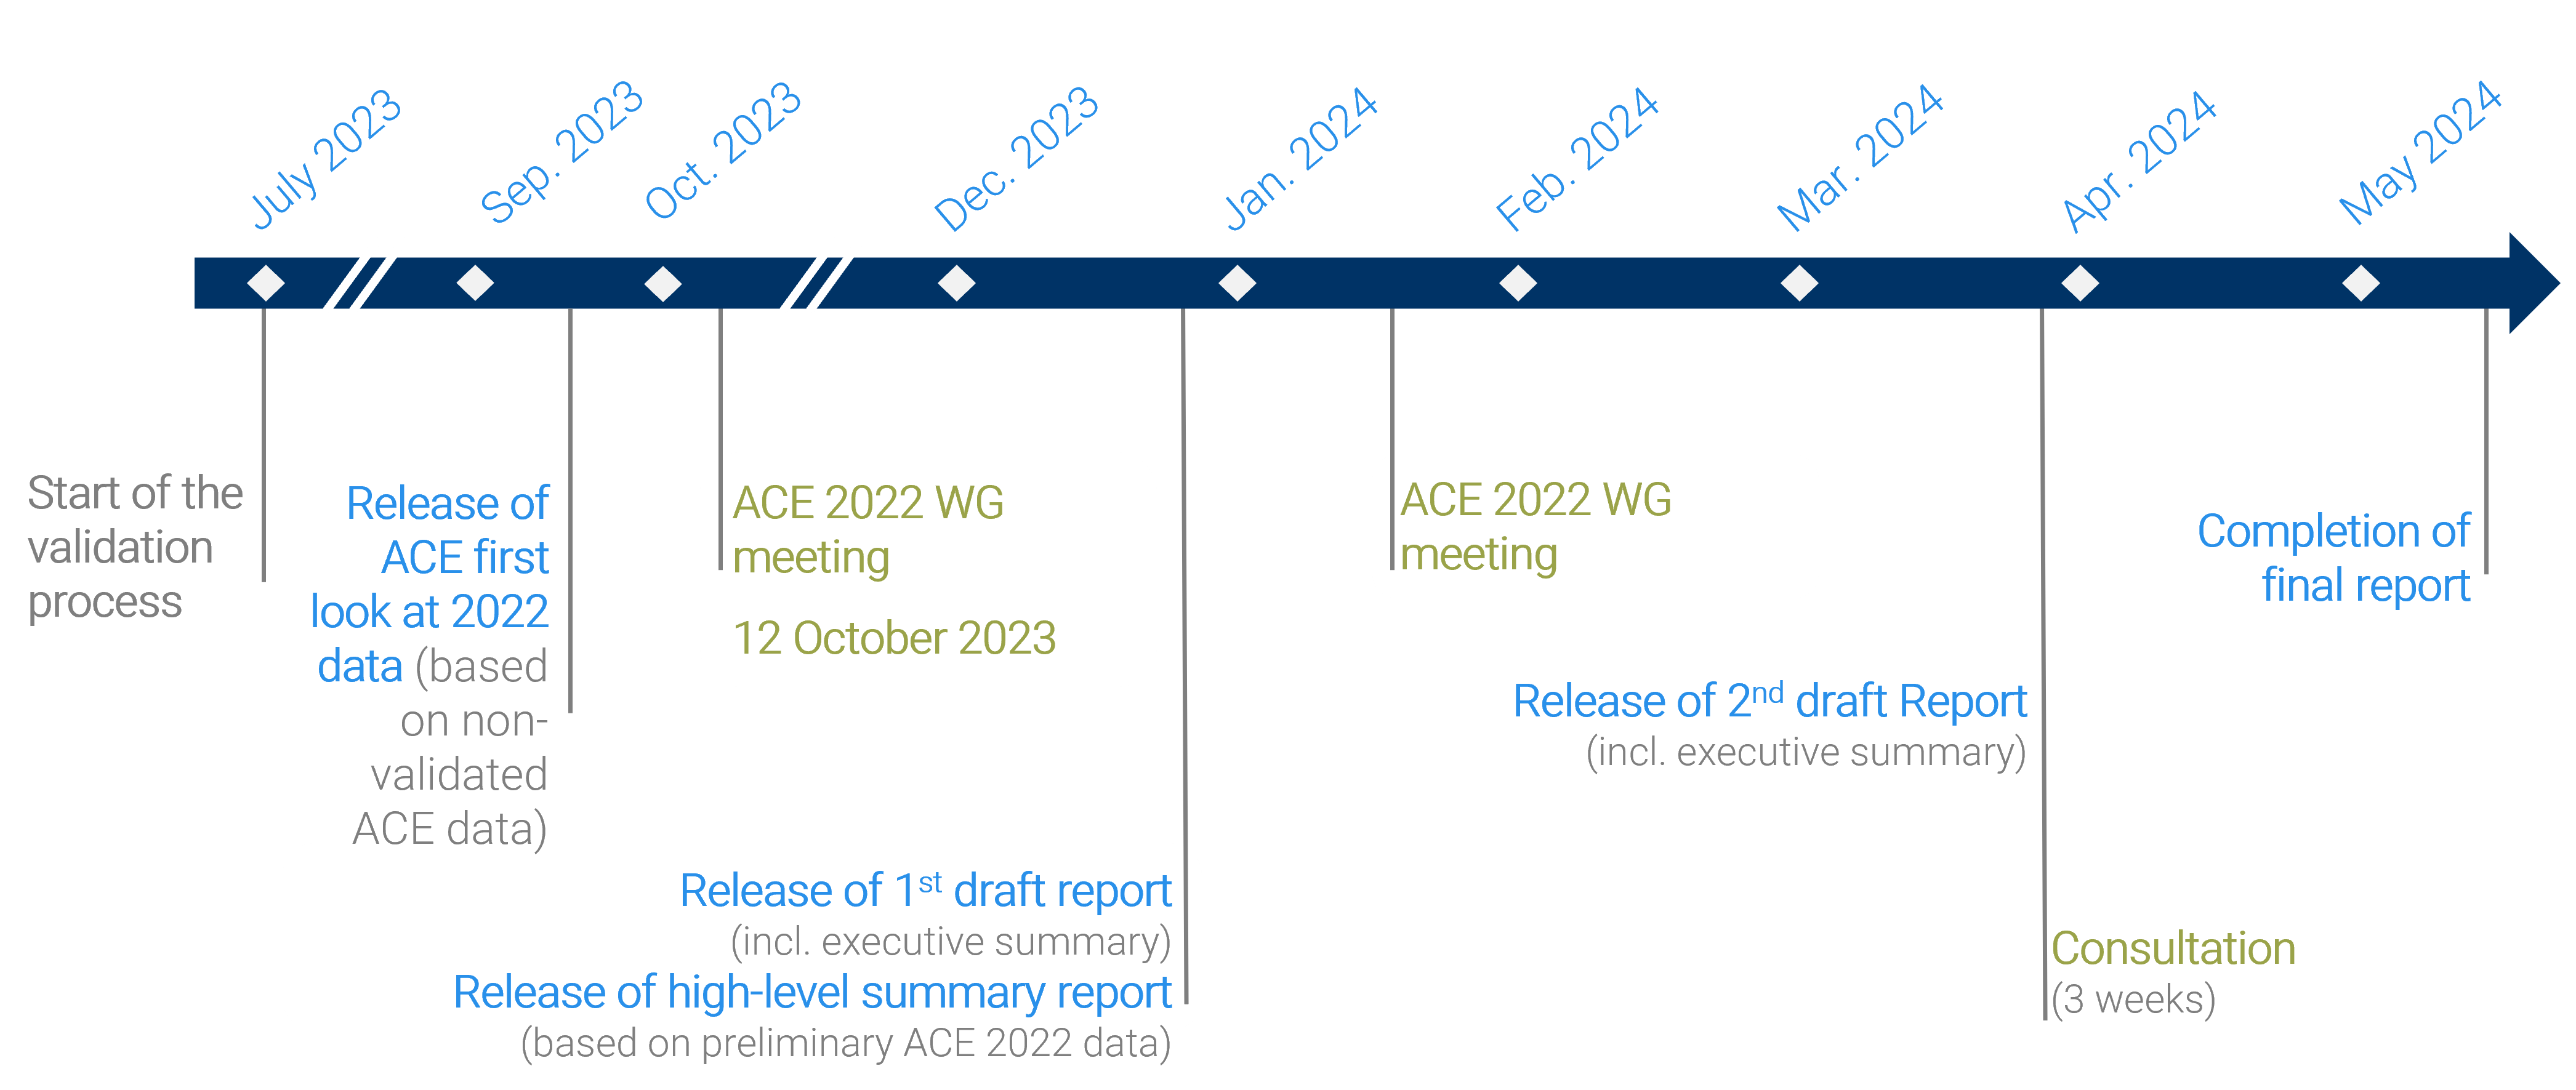
\includegraphics[width=0.8\linewidth]{figures/Figure-1-1} 

}

\caption{(ref:Figure-1-1)}\label{fig:Figure-1-1}
\end{figure}

It is important that robust ACE benchmarking analysis is available in a
timely manner since several stakeholders, most notably ANSPs'
management, regulatory authorities (e.g.~NSAs) and airspace users, have
a keen interest in receiving the information in the ACE reports as early
as possible.

It should be noted that the data presented in this document are still
preliminary and not yet fully validated. These data reflect the
information stored in the ACE database on the 11th November 2021. Figure
@ref(fig:Figure-1-2) shows the status of the ACE data validation process
for the data presented in this document.

(ref:Figure-1-2) Status of 2020 data validation process

\begin{figure}

{\centering 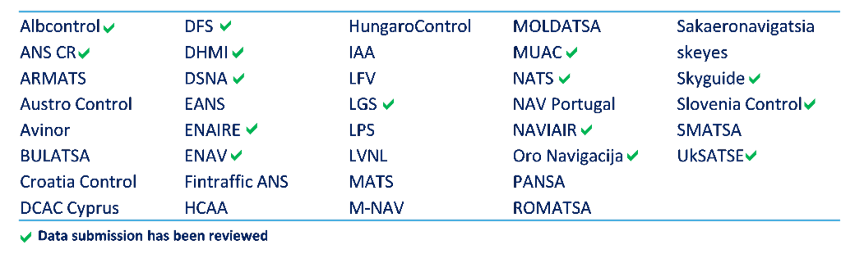
\includegraphics[width=0.8\linewidth]{figures/Figure-1-2} 

}

\caption{(ref:Figure-1-2)}\label{fig:Figure-1-2}
\end{figure}

The data contained in this report is therefore subject to changes before
the release of the final ACE 2020 benchmarking report in May 2022.

Figure @ref(fig:Figure-1-3) shows that 20 ANSPs provided their ACE 2020
data submission on time by the 1st July 2021 and that, in total, 26 data
submissions were received by the 15th July 2021. Figure
@ref(fig:Figure-1-3) also indicates that for 11 ANSPs the ACE data
submission was received more than one month after the deadline.

(ref:Figure-1-3) Status of ACE 2020 data submission

\begin{figure}

{\centering 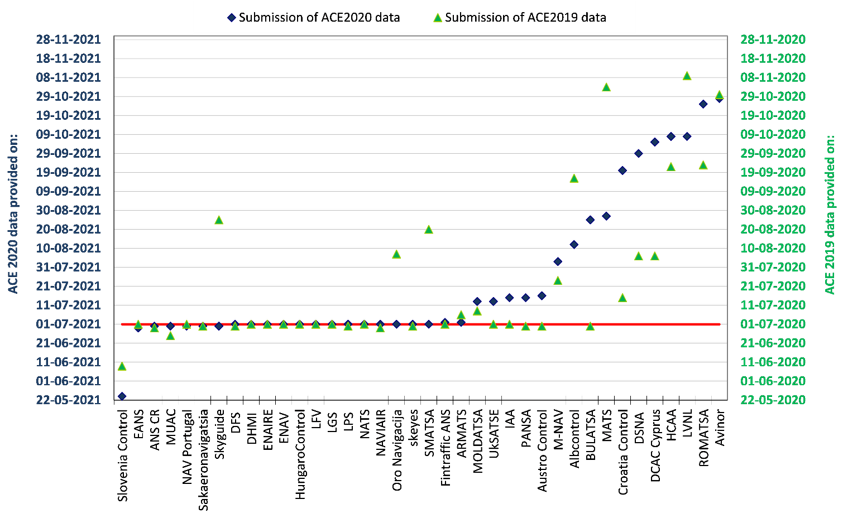
\includegraphics[width=0.8\linewidth]{figures/Figure-1-3} 

}

\caption{(ref:Figure-1-3)}\label{fig:Figure-1-3}
\end{figure}

Clearly, the timescale for the production of the ACE benchmarking report
is inevitably delayed if data are not submitted on time. The remainder
of this report is organised as follows:

\begin{itemize}
\tightlist
\item
  Section @ref(high): provides a high-level presentation of 2020
  revenues, costs and staff data;
\item
  Section @ref(economic): presents a preliminary analysis of economic
  cost-effectiveness at Pan-European and ANSP level;
\item
  Section @ref(financial): presents a preliminary analysis of financial
  cost-effectiveness at Pan-European and ANSP level, and underlying
  components.
\item
  Section @ref(covid): presents a preliminary analysis of specific
  financial indicators at Pan-European and ANSP level.
\end{itemize}

\hypertarget{high}{%
\chapter{High-level revenues, costs and staff data}\label{high}}

This section provides a preliminary presentation of high-level revenues,
costs and staff data provided in ANSPs ACE 2020 data submissions. Total
ANS revenues in 2020 amounted to €4 502M. Most en-route revenues come
from the collection of en-route charges (91.4\%, see left pie chart).
The proportion of terminal revenues from charges is lower (50.9\%, see
right pie chart), as additional income may directly come from airport
operators (31.2\% e.g.~through a contractual arrangement between the
ANSP and the airport operator).

(ref:Figure-2-1) Breakdown of gate-to-gate ANS revenues, 2020

\begin{figure}

{\centering 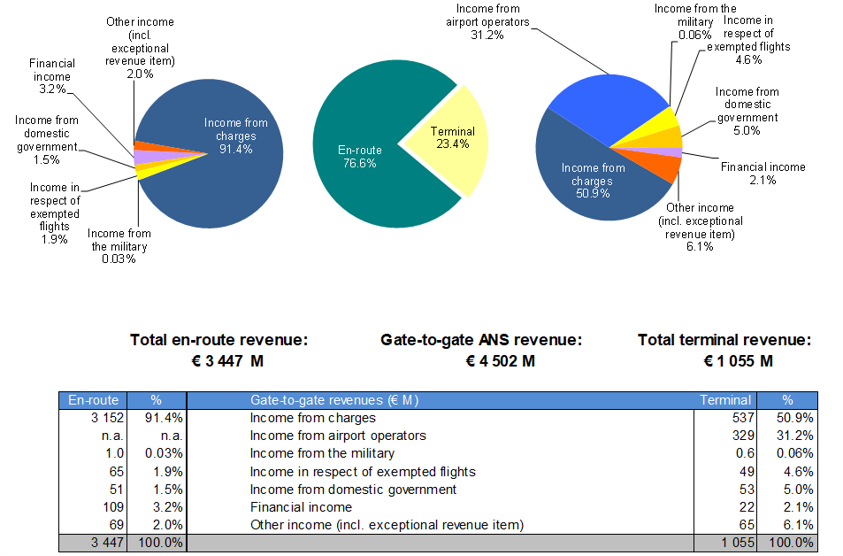
\includegraphics[width=0.8\linewidth]{figures/Figure-2-1} 

}

\caption{(ref:Figure-2-1)}\label{fig:Figure-2-1}
\end{figure}

Spotlight

Across the Pan-European system, traffic in 2020 (measured in composite
flight-hours) was -56.8\% lower than in 2019 and total gate-to-gate
revenues fell by -53.1\%. In this context there were also some changes
in the composition of ANSPs revenues, since the outbreak of COVID-19 did
not affect all sources of revenues in the same proportion.

Some revenue items increased in 2020, such as income from exempted
flights (+11.3\%), income from domestic governments (+11.3\%) and other
revenues (+21.6\%). However, these increases (+€46M) remain marginal
compared to the drop in en-route and terminal charges revenues (-€4 982
M) at Pan-European level. Detailed analysis shows that most ANSPs did
not record any State aid as part of their 2020 revenues.

At terminal level, the share of income from airport operator rose from
21.1\% in 2019 to 31.2\% in 2020 as this revenue stream reduced much
less than the income from terminal charges.

\begin{center}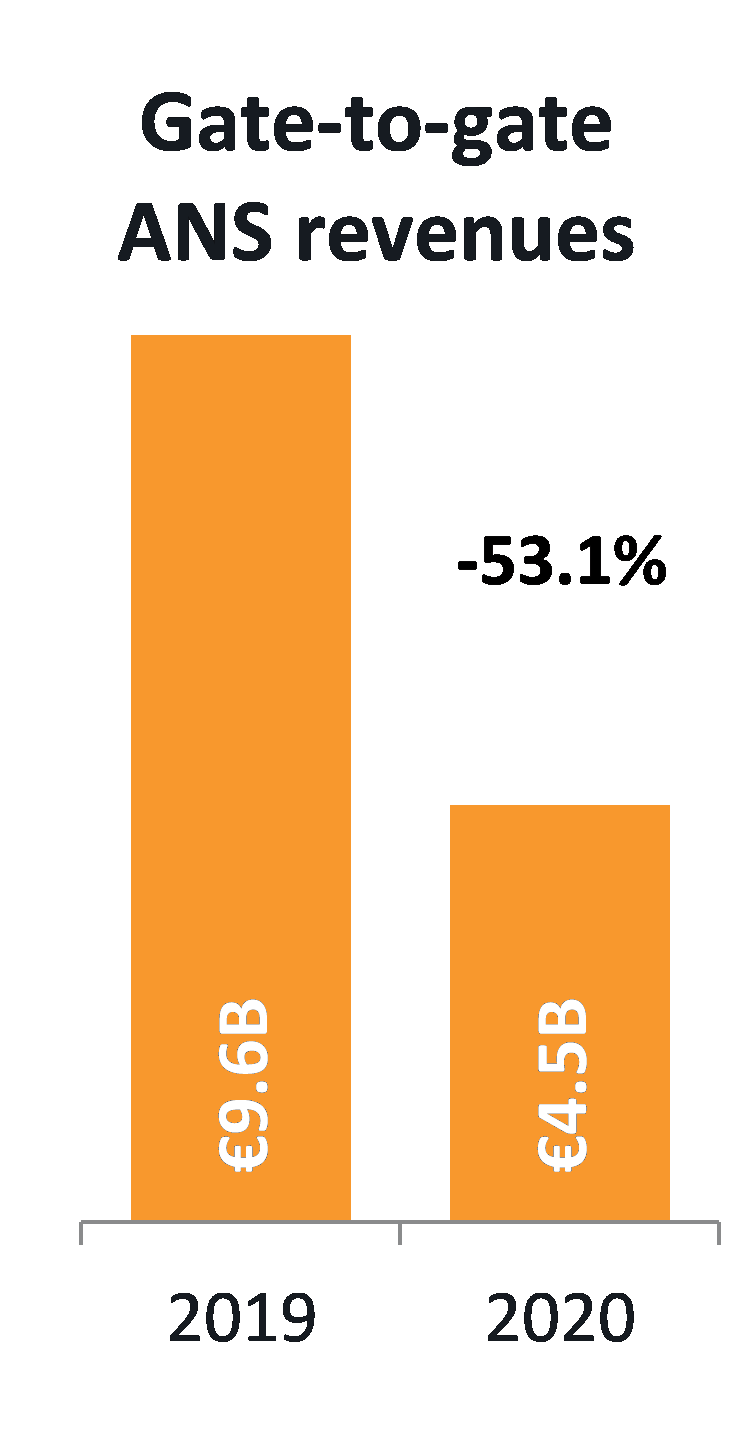
\includegraphics[width=0.8\linewidth]{figures/Figure-2-2} \end{center}

The ACE benchmarking analysis focuses on the specific costs of providing
gate-to-gate ATM/CNS services which amounted to €8 228M in 2020.
Operating costs (including staff costs, non-staff operating costs and
exceptional cost items) accounted for some 84\% of total ATM/CNS
provision costs, while depreciation costs and the cost of capital
represented some 16\%.

(ref:Figure-2-3) Gate-to-gate ATM/CNS provision costs at Pan-European
system level, 2020

\begin{figure}

{\centering 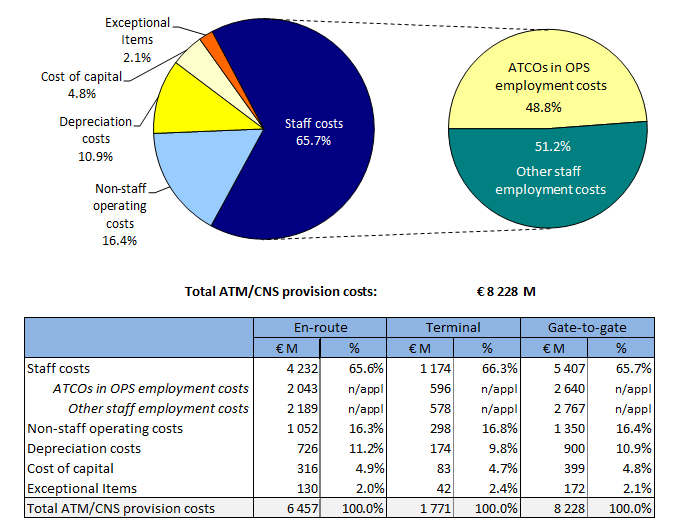
\includegraphics[width=0.7\linewidth]{figures/Figure-2-3} 

}

\caption{(ref:Figure-2-3)}\label{fig:Figure-2-3}
\end{figure}

In 2020, the five largest ANSPs (ENAIRE, ENAV, DFS, DSNA and NATS) bore
some 56\% of total Pan-European gate-to-gate ATM/CNS provision costs,
while the five smallest ANSPs accounted for some 1\% (see bottom left
part of Figure @ref(fig:Figure-2-5)).

ATM/CNS provision costs increased by +1.3\% p.a. between 2015 and 2019,
and then fell by -5.0\% in 2020 as ANSPs implemented a range of measures
to reduce costs and preserve liquidities. As shown in the bottom right
part of Figure @ref(fig:Figure-2-5), the -5.0\% decrease in ATM/CNS
costs in 2020 reflects reductions for 31 out of 38 ANSPs. More details
on the changes in ANSPs ATM/CNS provision costs in 2020 will be
available in the final ACE 2020 benchmarking report.

Spotlight

In response to the challenges presented by the extraordinary drop in
traffic, ANSPs implemented a range of cost-containment measures in 2020,
leading to an overall reduction in ATM/CNS costs of -€433.4M.

The full effect of these measures is however not yet visible in the 2020
data since, for instance, some redundancy plans were negotiated during
the year but the actual impact on the number of staff, and on the staff
costs, will become visible only in the 2021 data. Some ANSPs
implementing redundancy plans in 2020 even recorded cost increases in
the year, reflecting provisions or payments to the staff made redundant.
This was the main driver for an increase in exceptional costs of some
+€55.6M.

Staff costs were by far the main source of savings in 2020 (-€315.6M),
due to the implementation of the following measures:

\begin{itemize}
\tightlist
\item
  Short-time work / furlough schemes, where applicable, with part of
  employees' salaries paid by the State either directly to the employees
  or reducing ANSPs wage bill.
\item
  Reduced staff numbers (discussed further below).
\item
  Reduced level of remuneration through reduction or freeze of base
  salaries, reduction or suspension of variable part of salaries such as
  overtime payments and performance bonuses.
\end{itemize}

A majority of ANSPs also reduced non-staff operating costs by carrying
out only essential maintenance, reducing utilities costs and
non-essential training activities. This resulted in a decrease of some
-€39.2M.

Finally, the cancellation or deferral of non-essential investments
resulted in lower depreciation costs (-€51.0M) and lower cost of capital
(-€83.2M). The latter is also impacted, in many cases, by the use of a
lower weighted average cost of capital in 2020.

\begin{center}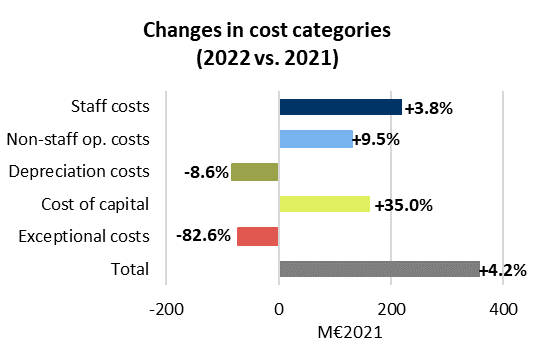
\includegraphics[width=1\linewidth]{figures/Figure-2-4} \end{center}

(ref:Figure-2-5) Changes in ATM/CNS provision costs, 2015-2020 (real
terms)

\begin{figure}

{\centering 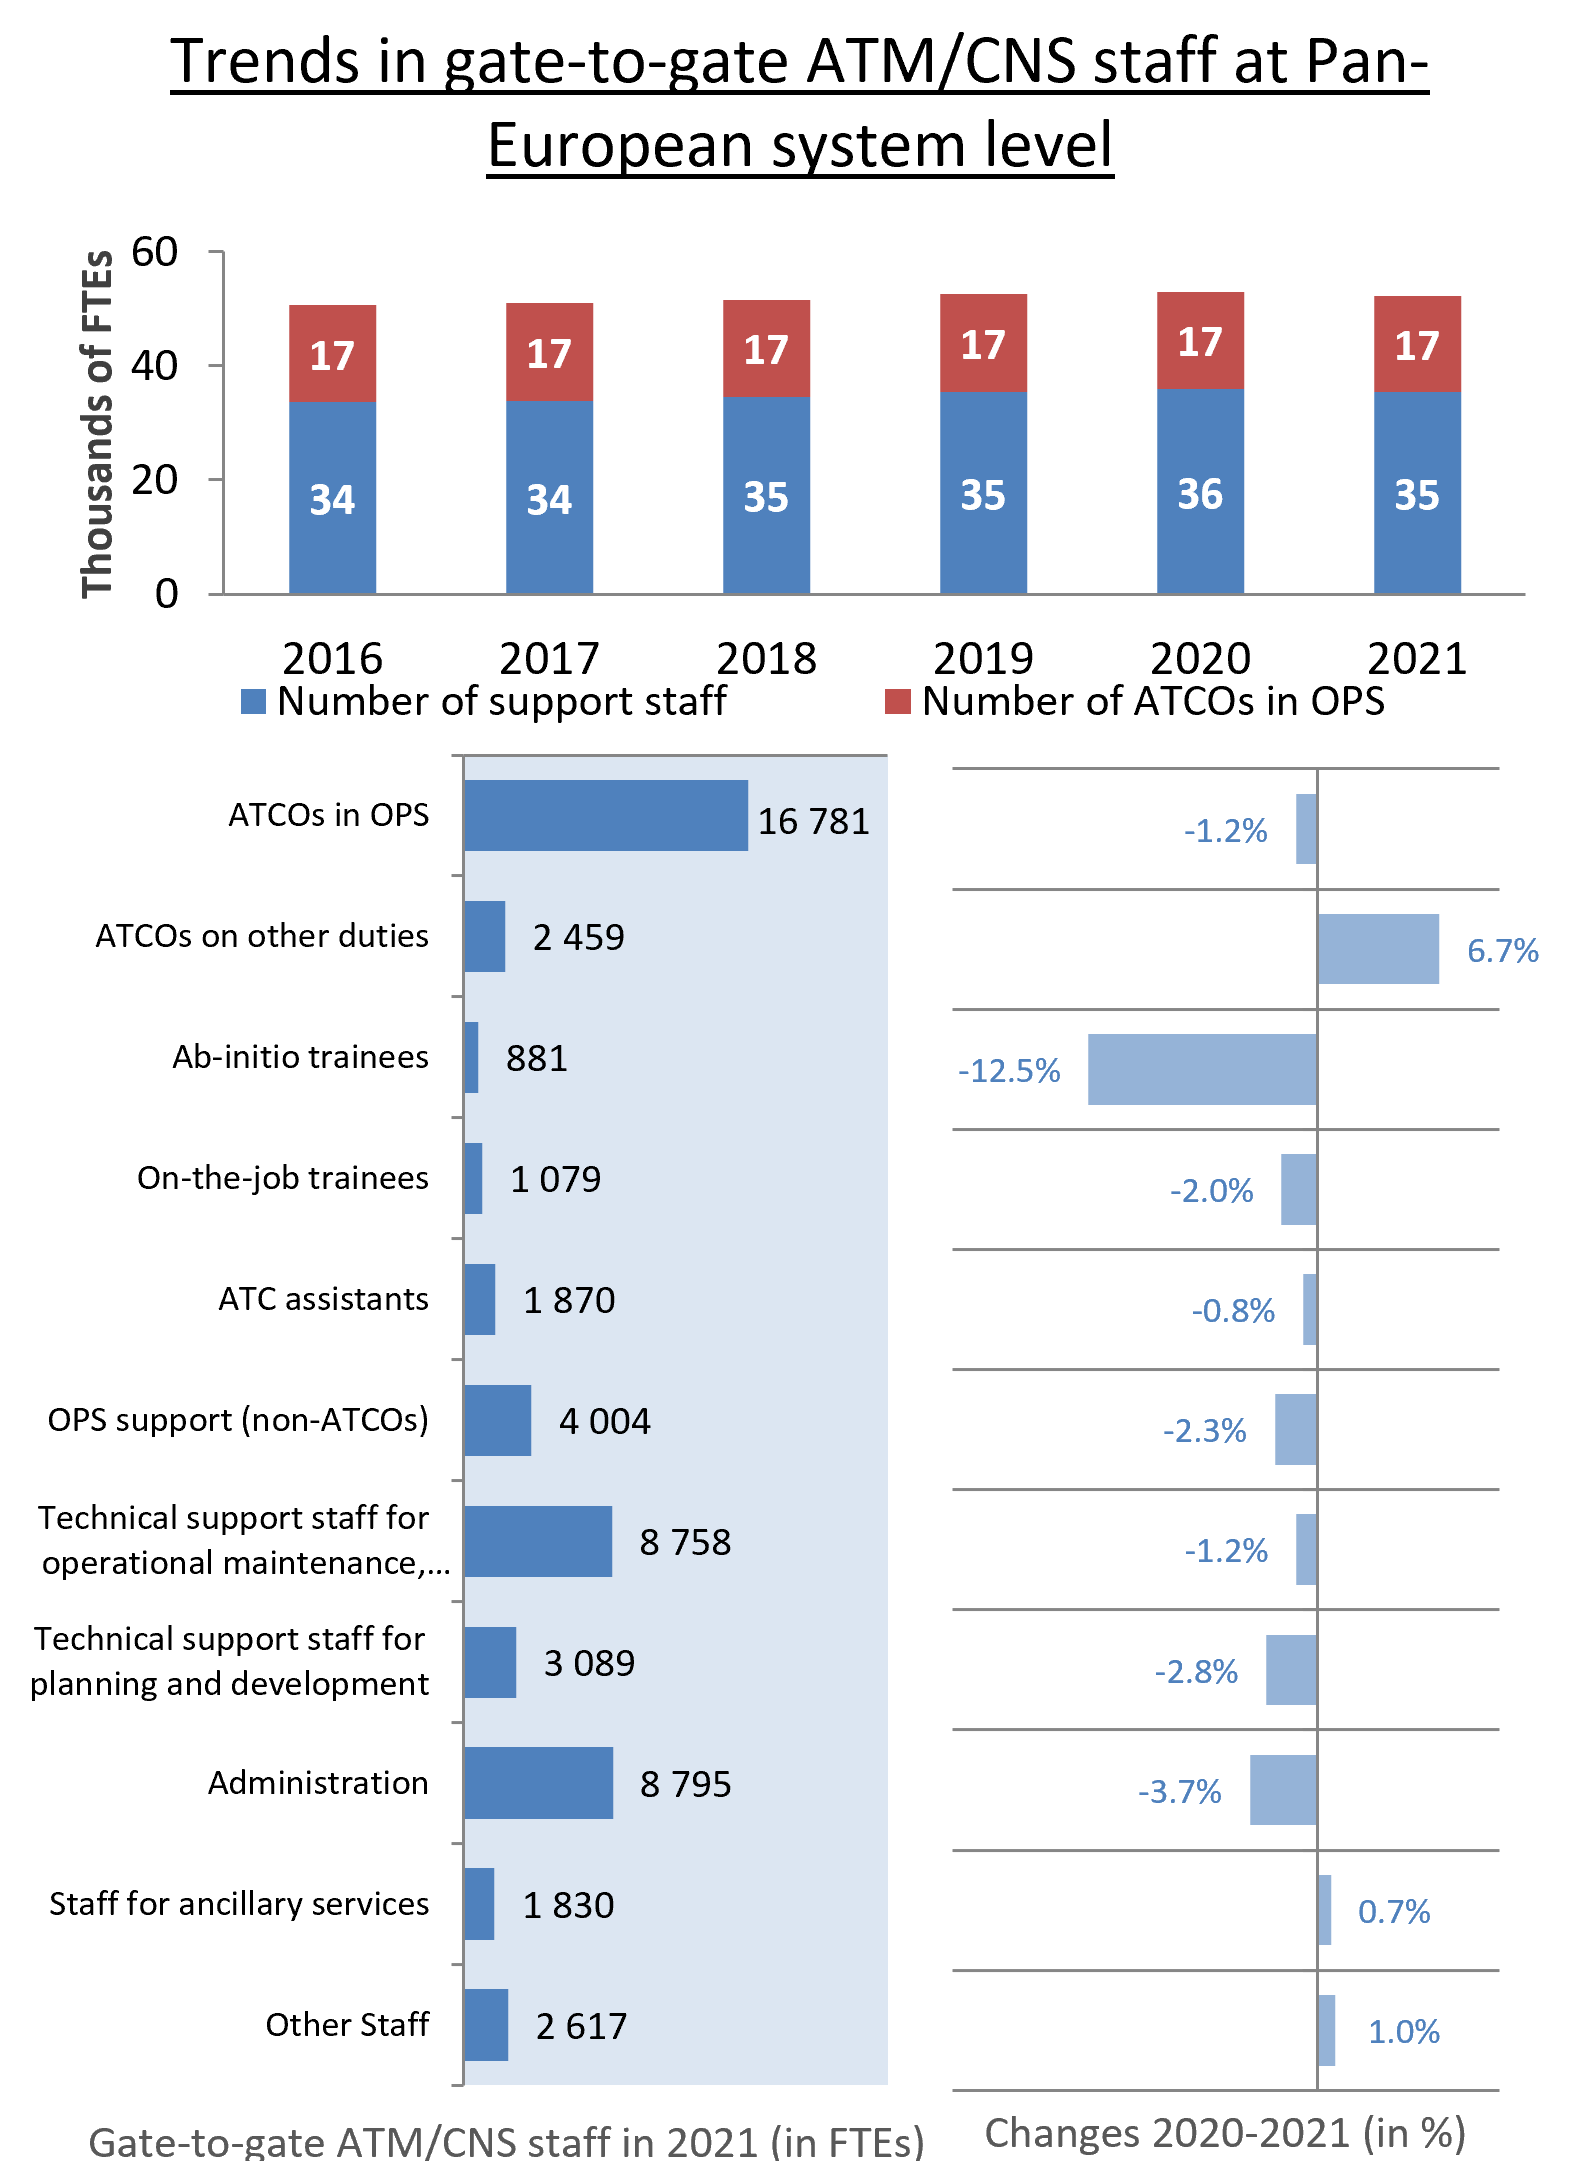
\includegraphics[width=0.7\linewidth]{figures/Figure-2-5} 

}

\caption{(ref:Figure-2-5)}\label{fig:Figure-2-5}
\end{figure}

The Pan-European employed a total of 55 712 staff in 2020 (comprising 54
871 staff providing ATM/CNS services and 845 internal MET staff). Some
17 400 staff (32\%) were ATCOs working on operational duty, split
between ACCs (56\%) and APP/TWR facilities (44\%). On average, 2.2
additional staff are required for every ATCO in OPS in Europe.

(ref:Figure-2-6) Breakdown of total gate-to-gate ATM/CNS staff at
Pan-European system level, 2020

\begin{figure}

{\centering 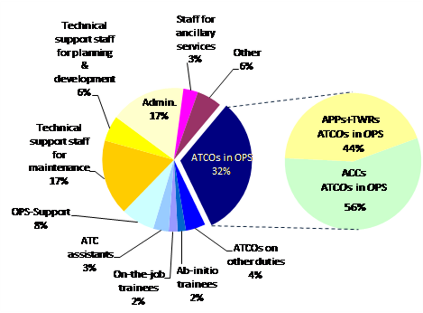
\includegraphics[width=0.6\linewidth]{figures/Figure-2-6} 

}

\caption{(ref:Figure-2-6)}\label{fig:Figure-2-6}
\end{figure}

(ref:Figure-2-7) Total gate-to-gate ATM/CNS staff per staff category and
changes, 2019-2020

\begin{figure}

{\centering 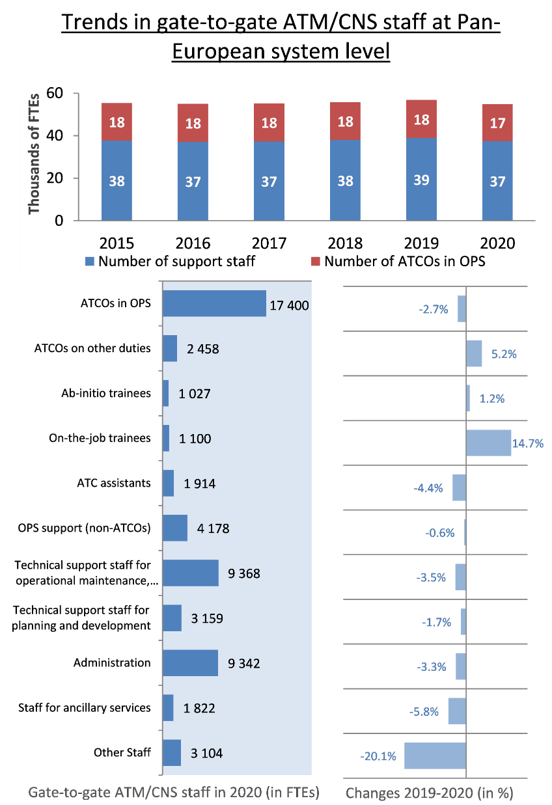
\includegraphics[width=0.7\linewidth]{figures/Figure-2-7} 

}

\caption{(ref:Figure-2-7)}\label{fig:Figure-2-7}
\end{figure}

After four years of continuous increase in the number of ATM/CNS staff
(+0.6\% p.a. between 2015 and 2019, or +1 384 FTEs), 2020 showed a
-3.4\% reduction (-1 936 FTEs).

The lower staff number observed for 2020 mainly reflects decreases in
the following staff categories:

\begin{itemize}
\tightlist
\item
  Other staff (-779 FTEs or -20.1\%);
\item
  ATCOs in OPS (-485 FTEs, or -2.7\%);
\item
  Technical support for operational maintenance (-340 FTEs, or -3.5\%);
\item
  Administrative staff (-323 FTEs, or -3.3\%); and,
\item
  Staff for ancillary services (-112 FTEs or -5.8\%).
\end{itemize}

On the other hand, increases are observed for ATCOs on other duties
(+121 FTEs) and on-the-job trainees (+141 FTEs), reflecting a
reallocation of some ATCOs from operational to non-operational duties
due to the traffic reduction in 2020, and the fact that newly recruited
ATCOs had to complete their on-the-job training.

Spotlight

In addition to the measures on staff costs already mentioned above
(redundancies, short-time work / furlough schemes), it is important to
note that during the lockdown periods, some ANSPs staff had to consume
accumulated holidays not used in previous years and/or made use of
pre-retirement schemes. Furthermore, depending on the nature of their
work, some staff were inevitably left without specific tasks, however,
in most cases, they continued to be counted as full time equivalents in
2020.

It is also important to note that the trend observed at Pan-European
system level is heavily affected by the reporting of very large
reductions by UkSATSE. Excluding UkSATSE, the total number of ATM/CNS
staff in 2020 would be close to its 2019 level (-0.1\%).

The trends shown in the Figure @ref(fig:Figure-2-7) above should
therefore be interpreted with caution.

Although some ANSPs might have discontinued the ATCO recruitment process
during the pandemic, the number of ab-initio trainees increased by
+1.2\% in 2020. It will be interesting to monitor this trend in future
years as the long time period required to train a fully qualified ATCO
might have an impact on the level the capacity offered by ANSPs when
traffic returns to pre-crisis levels.

\hypertarget{economic}{%
\chapter{Economic cost-effectiveness}\label{economic}}

The PRC introduced in its ACE benchmarking reports the concept of
economic cost-effectiveness. This indicator is defined as gate-to-gate
ATM/CNS provision costs plus the costs of ground ATFM delays for both
en‐route and airport, all expressed per composite flight-hour. This
economic performance indicator is meant to capture trade‐offs between
ATC capacity and costs\footnote{See Annex 2 of the ACE 2019 benchmarking
  report for more information on the methodology used to compute
  composite flight-hours and economic costs.}.

Figure @ref(fig:Figure-3-1) shows preliminary results on the changes in
economic cost-effectiveness between 2015 and 2020 at Pan-European system
level. The left-hand side of Figure @ref(fig:Figure-3-1) shows the
changes in unit economic costs, while the right-hand side provides
complementary information on the year-on-year changes in ATM/CNS
provision costs, composite flight-hours and unit costs of ATFM delays.

(ref:Figure-3-1) Trend of unit economic costs at Pan-European system
level, 2015-2020 (real terms)

\begin{figure}

{\centering 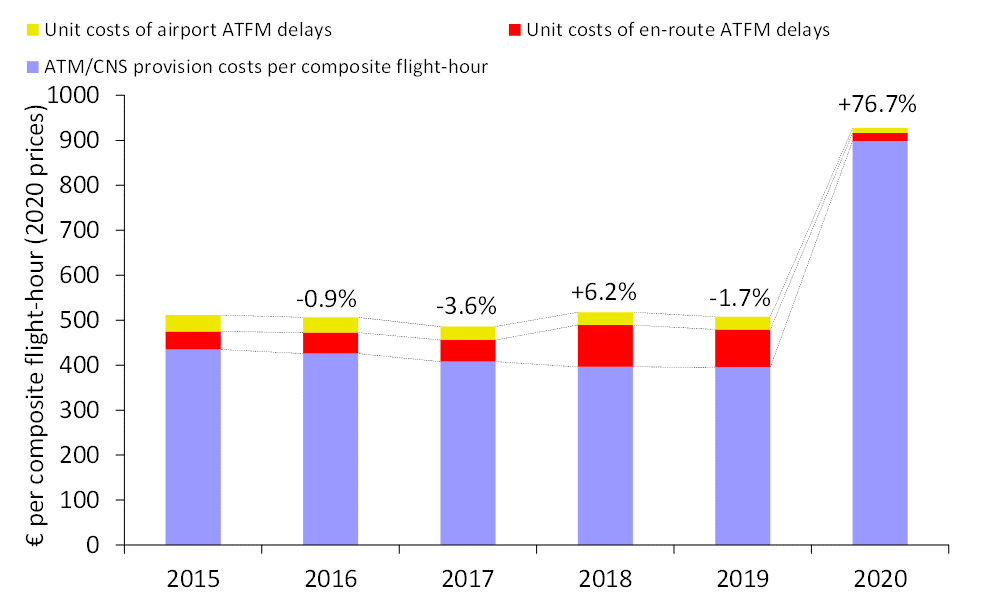
\includegraphics[width=0.5\linewidth]{figures/Figure-3-1-Left} 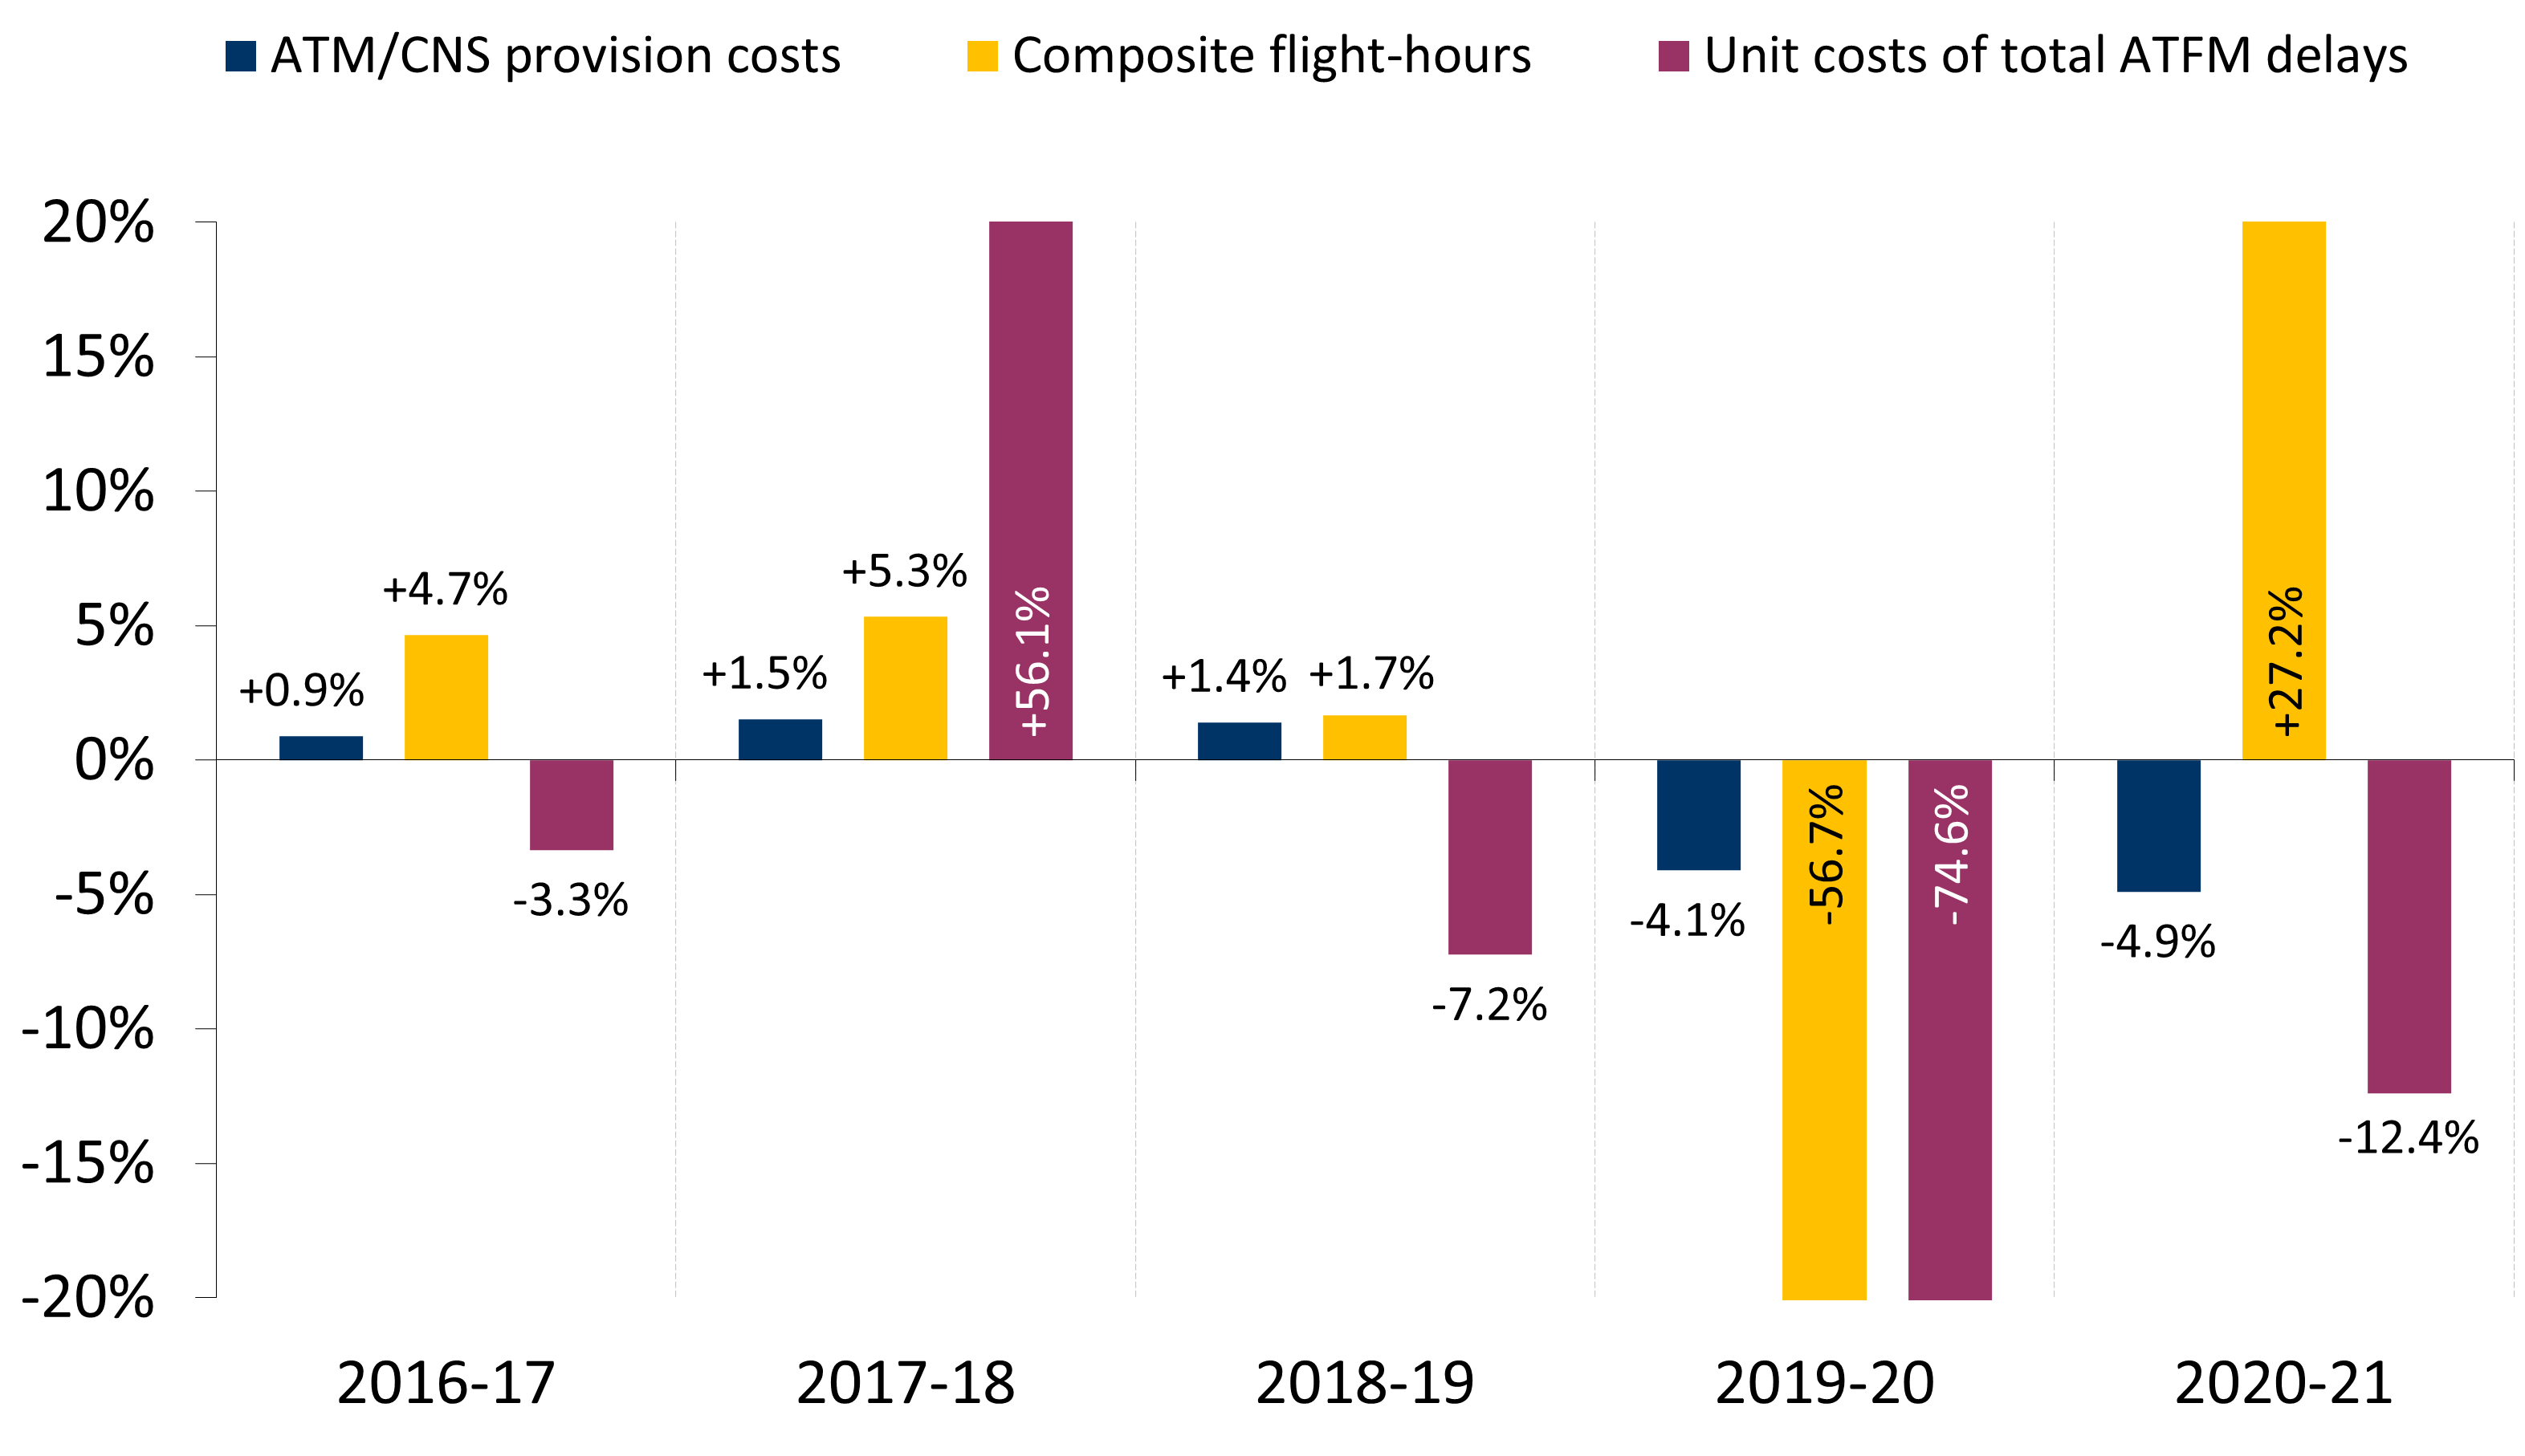
\includegraphics[width=0.5\linewidth]{figures/Figure-3-1-Right} 

}

\caption{(ref:Figure-3-1)}\label{fig:Figure-3-1}
\end{figure}

Figure @ref(fig:Figure-3-2) shows preliminary results at ANSP level
(dotted lines represent the 1st and 3rd quartiles). On average, the
share of ATFM delays in 2020 was 3\% (compared to 22\% in 2019), and
only five ANSPs had ATFM delays representing more than 5\% of their unit
economic costs (compared to 22 ANSPs in 2019).

(ref:Figure-3-2) Economic gate-to-gate cost-effectiveness, 2020

\begin{figure}

{\centering 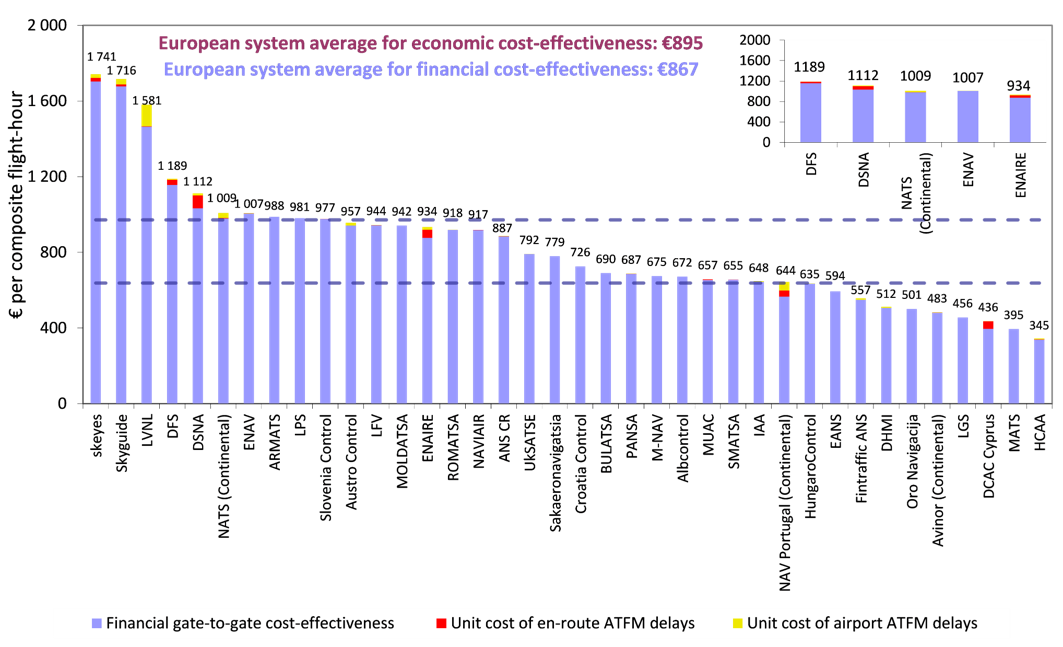
\includegraphics[width=1\linewidth]{figures/Figure-3-2} 

}

\caption{(ref:Figure-3-2)}\label{fig:Figure-3-2}
\end{figure}

\hypertarget{financial}{%
\chapter{Financial cost-effectiveness}\label{financial}}

This section provides a preliminary analysis of financial
cost-effectiveness.

\hypertarget{fin_1}{%
\section{Pan-European system level}\label{fin_1}}

Figure @ref(fig:Figure-4-1) shows that after three years of continuous
reductions and a stabilization in 2019, the unit ATM/CNS provision costs
rose by +120.0\% in 2020. This extraordinary increase is mainly due to
the decrease in composite flight-hours (-56.8\%) while ATM/CNS provision
costs fell by -5.0\%.

The analytical framework which is used in the ACE analysis to break down
the financial cost-effectiveness indicator into basic economic drivers
is presented in Figure @ref(fig:Figure-4-2). These key drivers include:

\begin{enumerate}
\def\labelenumi{\alph{enumi})}
\tightlist
\item
  ATCO-hour productivity (0.47 composite flight-hours per ATCO-hour);
\item
  ATCO employment costs per ATCO-hour (€131); and,
\item
  Support costs per unit output (€589).
\end{enumerate}

(ref:Figure-4-1) Changes in unit ATM/CNS provision costs, 2015-2020
(real terms)

\begin{figure}

{\centering 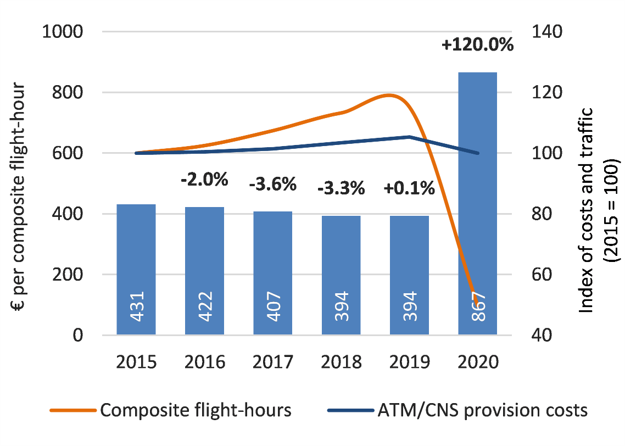
\includegraphics[width=0.7\linewidth]{figures/Figure-4-1} 

}

\caption{(ref:Figure-4-1)}\label{fig:Figure-4-1}
\end{figure}

Figure @ref(fig:Figure-4-2) shows that in 2020, ATCO employment costs
per ATCO-hour rose by +12.2\% while ATCO-hour productivity fell by
-49.0\%. As a result, ATCO employment costs per composite flight-hour
increased (+120.1\%).

In the meantime, unit support costs rose by +120.0\% since the fall in
composite flight-hours (-56.8\%) was much greater than the reduction in
support costs (-5.0\%). As a result, in 2020 unit ATM/CNS provision
costs increased by +120.0\% at Pan-European system level.

(ref:Figure-4-2) ACE performance framework, 2020 (real terms)

\begin{figure}

{\centering 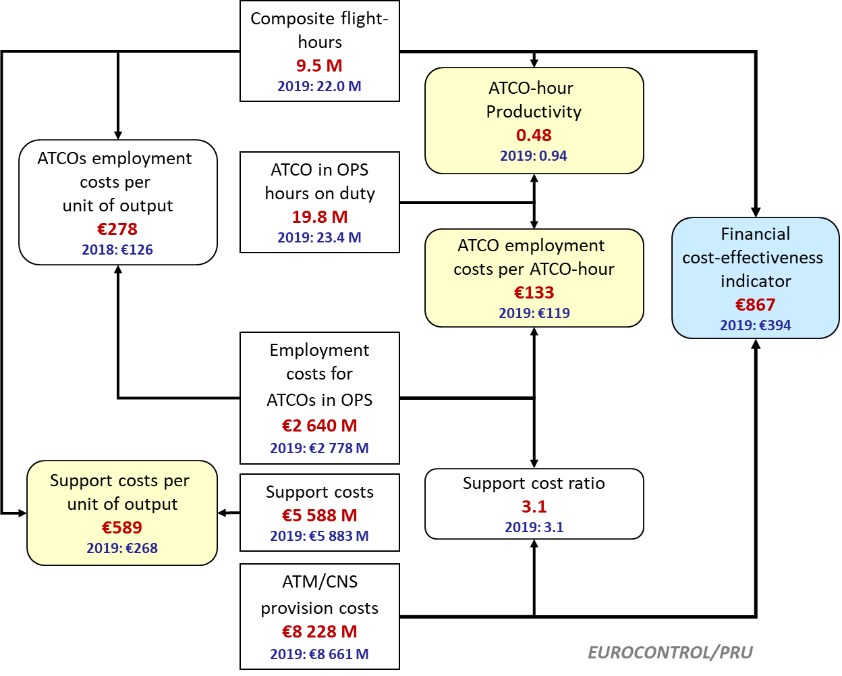
\includegraphics[width=0.7\linewidth]{figures/Figure-4-2} 

}

\caption{(ref:Figure-4-2)}\label{fig:Figure-4-2}
\end{figure}

(ref:Figure-4-3) Breakdown of changes in unit ATM/CNS provision costs,
2019-2020 (real terms)

\begin{figure}

{\centering 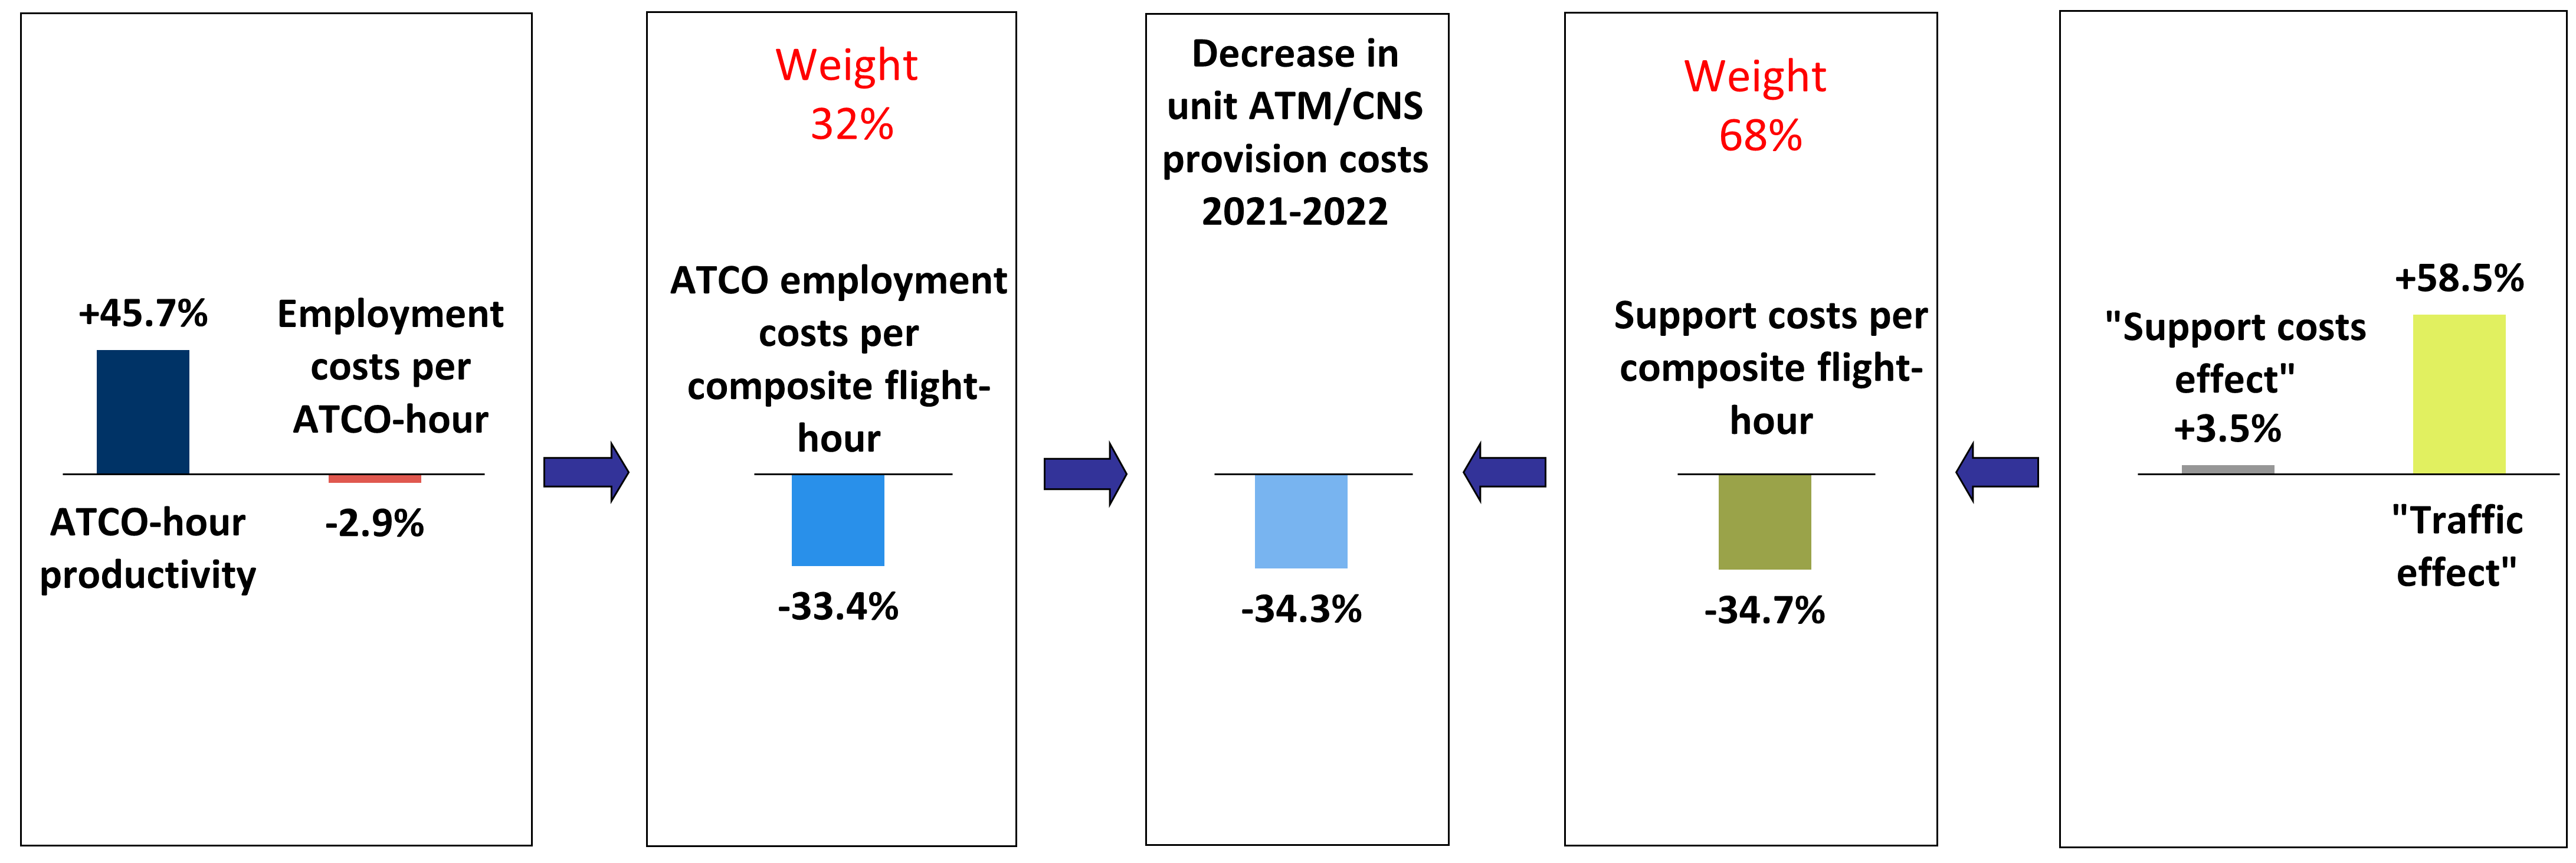
\includegraphics[width=0.8\linewidth]{figures/Figure-4-3} 

}

\caption{(ref:Figure-4-3)}\label{fig:Figure-4-3}
\end{figure}

\hypertarget{fin_2}{%
\section{ANSP level}\label{fin_2}}

Figure @ref(fig:Figure-4-4) to Figure @ref(fig:Figure-4-7) present the
main ACE key performance indicators at ANSP level for the year 2020. In
all these figures, the dotted lines represent the 1st and 3rd quartiles.

There are three main elements to be considered when interpreting the
level of the indicators as well as ANSPs rankings in the figures below:
a) the traffic reduction in 2020, although being massive for all ANSPs,
was not completely homogeneous, b) there were different responses in
cost adjustments, and c) there were also different levels of flexibility
in adjusting the workforce, and in particular ATCO in OPS hours on duty,
which has an enormous impact on the ATCO productivity and employment
costs indicators measured in the ACE report.

(ref:Figure-4-4) Financial gate-to-gate cost-effectiveness, 2020

\begin{figure}

{\centering 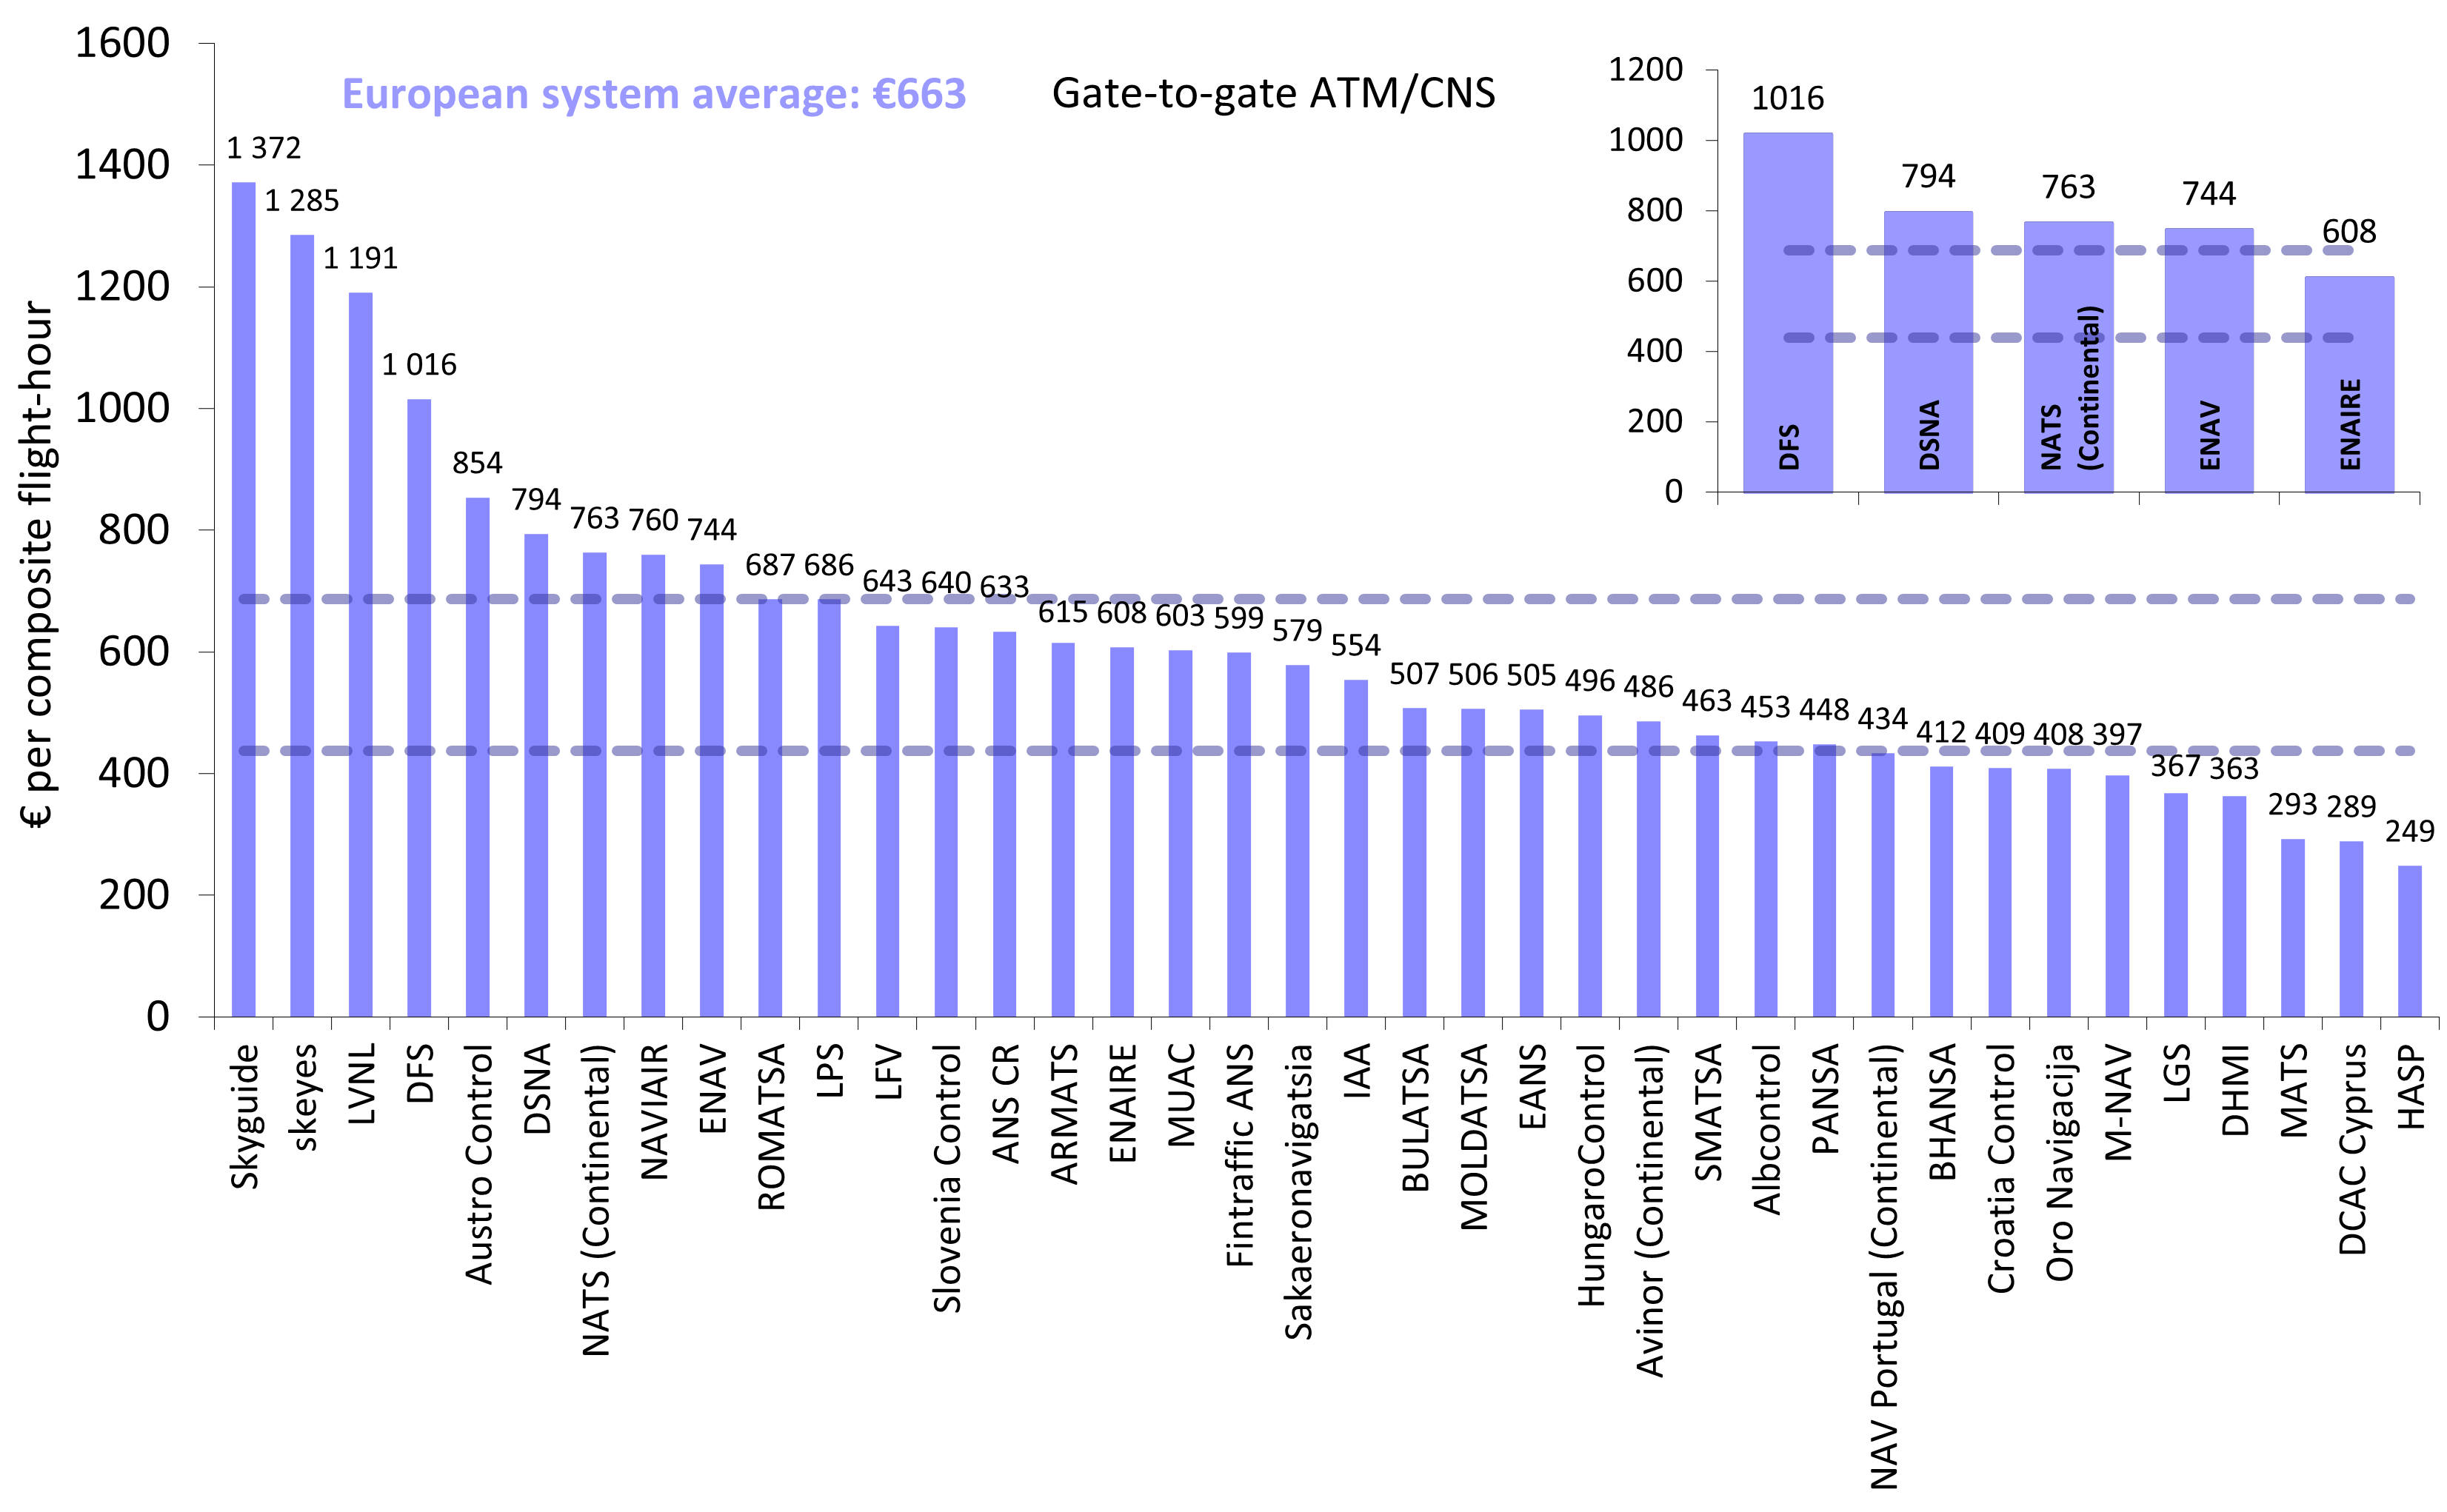
\includegraphics[width=0.8\linewidth]{figures/Figure-4-4} 

}

\caption{(ref:Figure-4-4)}\label{fig:Figure-4-4}
\end{figure}

(ref:Figure-4-5) ATCO-hour productivity, 2020

\begin{figure}

{\centering 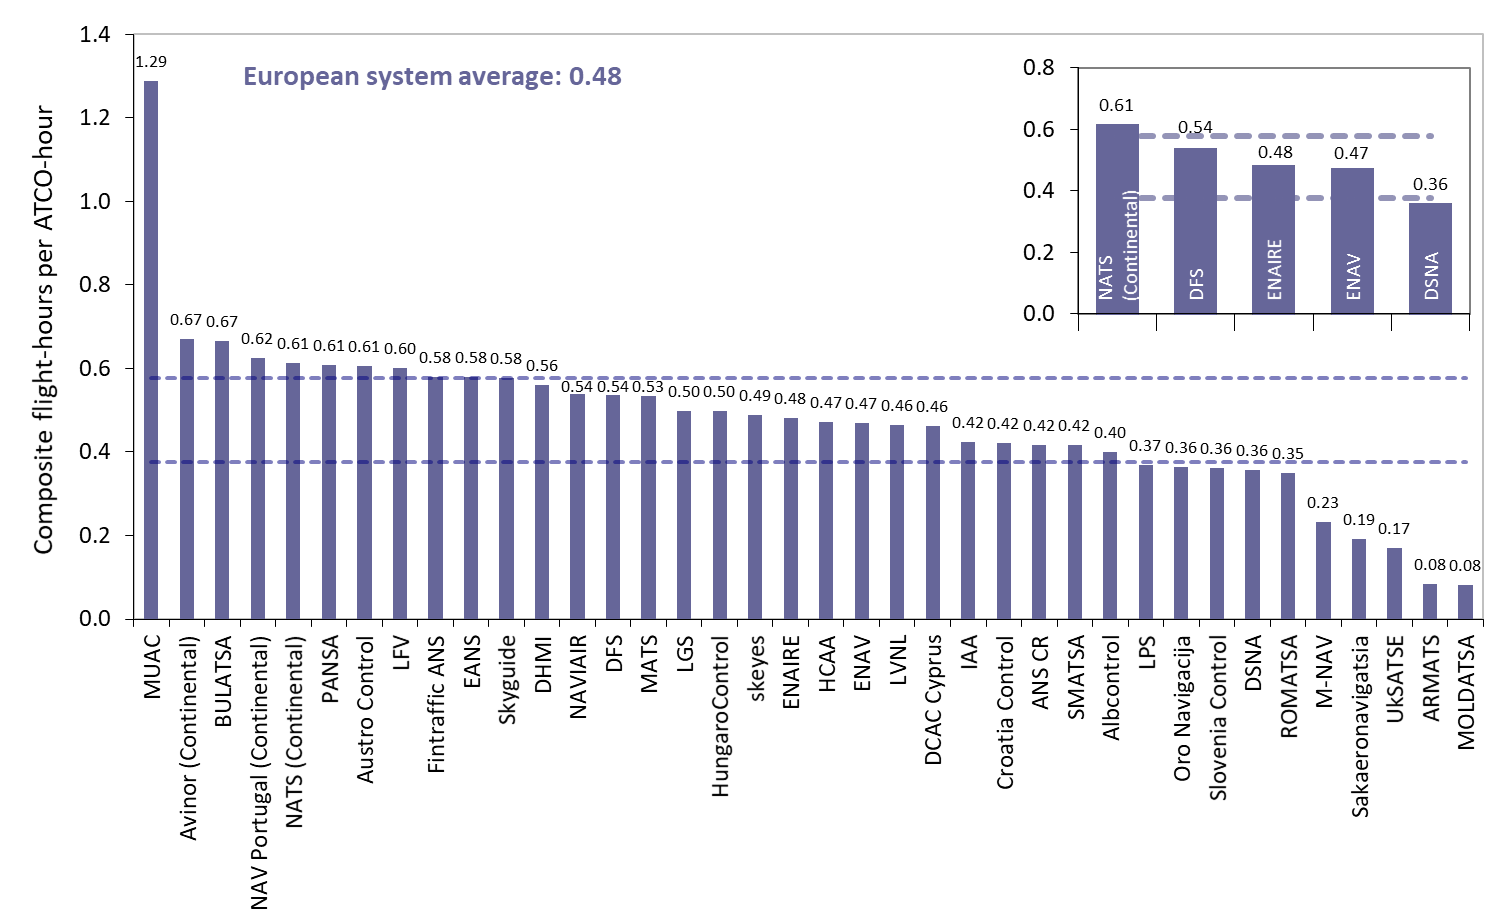
\includegraphics[width=0.8\linewidth]{figures/Figure-4-5} 

}

\caption{(ref:Figure-4-5)}\label{fig:Figure-4-5}
\end{figure}

(ref:Figure-4-6) Employment costs per ATCO-hour, 2020

\begin{figure}

{\centering 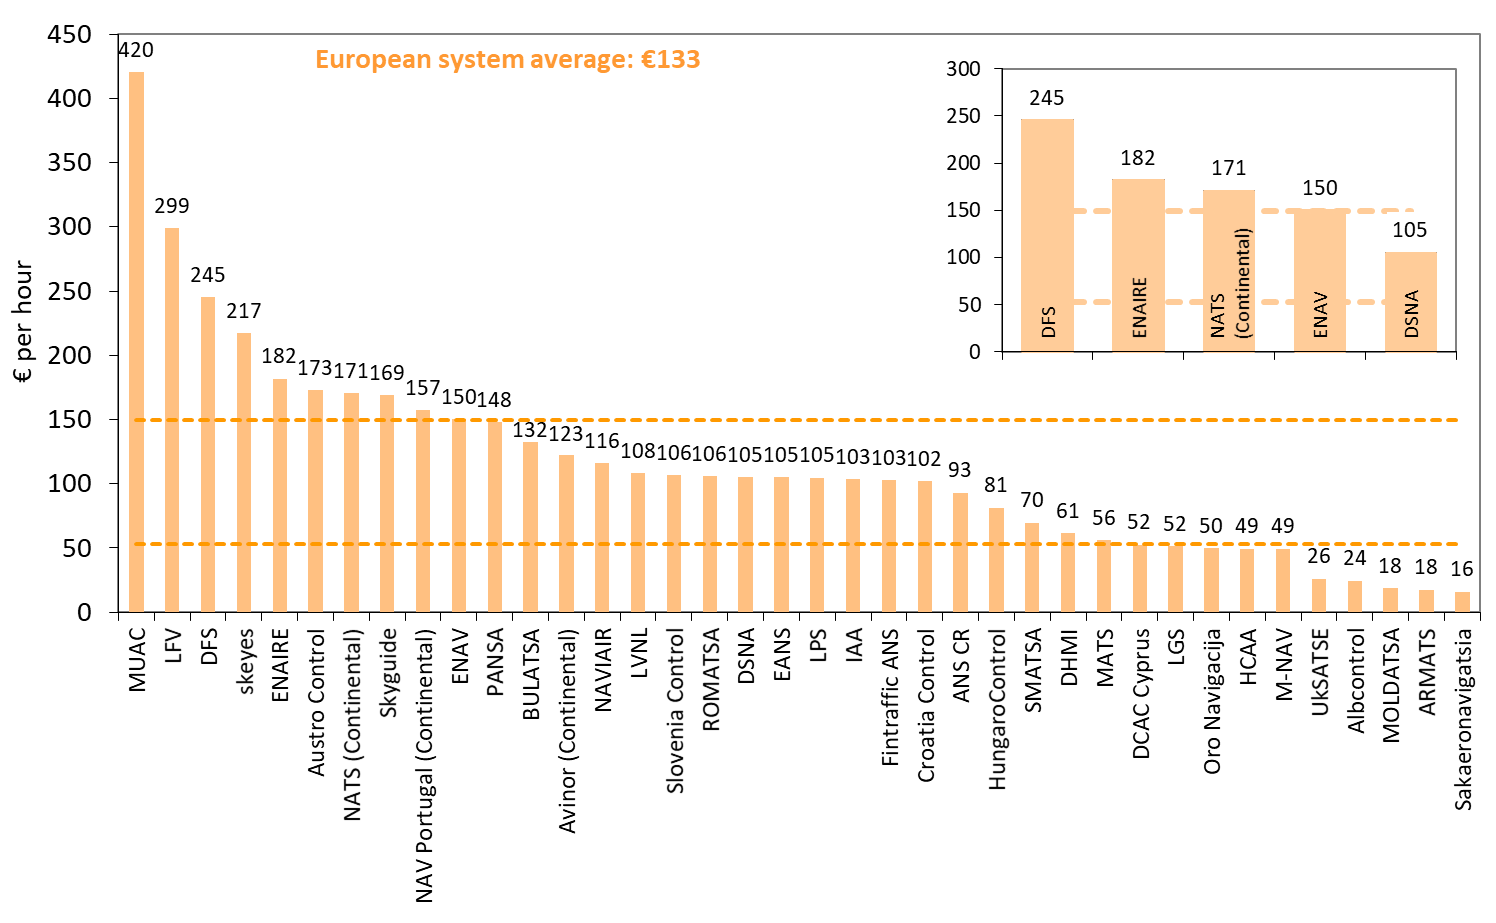
\includegraphics[width=0.8\linewidth]{figures/Figure-4-6} 

}

\caption{(ref:Figure-4-6)}\label{fig:Figure-4-6}
\end{figure}

(ref:Figure-4-7) Breakdown of support costs per composite flight-hour,
2020

\begin{figure}

{\centering 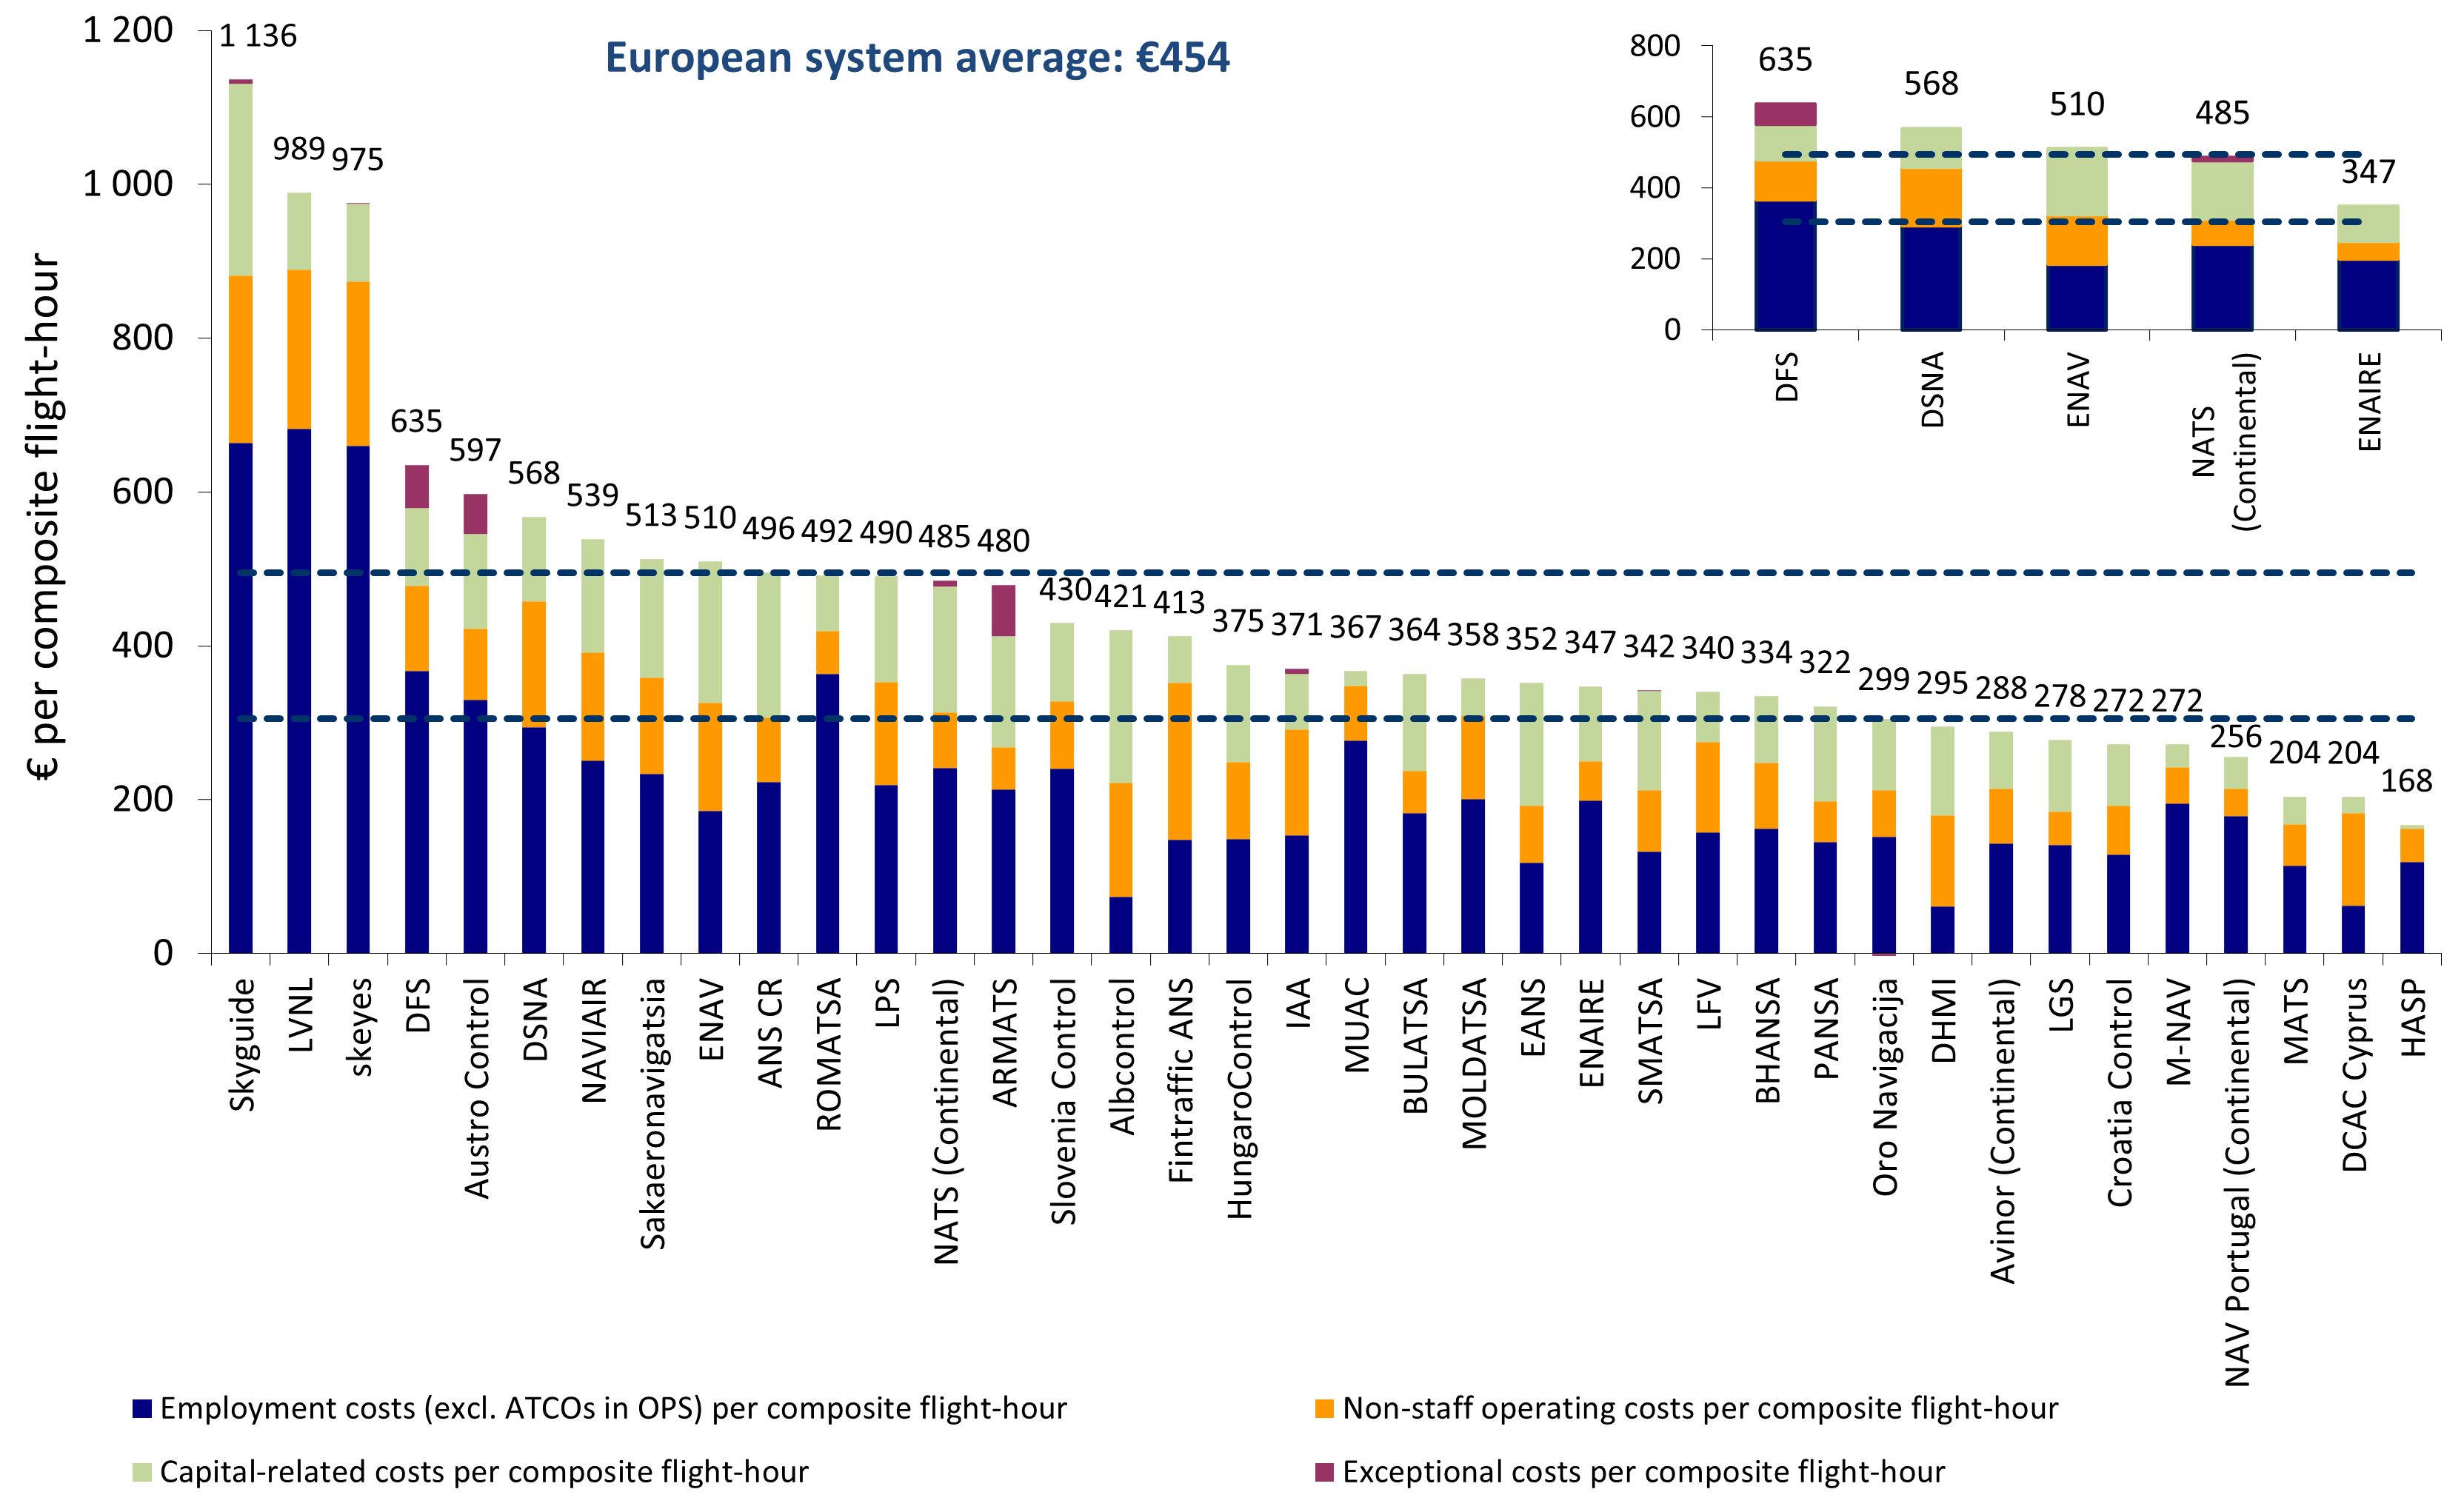
\includegraphics[width=0.8\linewidth]{figures/Figure-4-7} 

}

\caption{(ref:Figure-4-7)}\label{fig:Figure-4-7}
\end{figure}

A more detailed analysis of the changes in cost-effectiveness, ATCO-hour
productivity, ATCO employment costs per ATCO-hour and unit support costs
will be available in the final ACE 2020 benchmarking report.

\hypertarget{covid}{%
\chapter{ANSPs Cash and Liquidity Issues as a Result of the Covid-19
Pandemic}\label{covid}}

This section provides a preliminary analysis of specific financial
indicators that can be used to monitor potential cash and liquidity
issues experienced by ANSPs as a result of the COVID-19 pandemic. It is
structured into three parts:

\begin{itemize}
\tightlist
\item
  changes in ANSPs balance sheet structure at Pan-European system level
  between 2019 and 2020;
\item
  presentation of three financial indicators that can be calculated from
  ACE data submissions (current ratio, cash-on-hand days and equity
  ratio); and,
\item
  presentation of the free cash flow indicator, which is calculated from
  ANSPs financial statements.
\end{itemize}

Due to specific organisational and financial set up in HCAA, LVNL and
MUAC, these three ANSPs are excluded from the analysis presented in this
section.

\hypertarget{covid_1}{%
\section{Changes in the balance sheet structure}\label{covid_1}}

Figure @ref(fig:Figure-5-1) presents the changes in ANSPs balance sheet
structure as reported in their ACE data submissions at ``Total ANS''
level (i.e.~en-route, terminal and other ANS). The scope is therefore
wider than gate-to-gate ATM/CNS which is used to calculate the other ACE
key performance indicators, but depending on what ANSPs include under
``Other ANS,'' it might not necessarily match with the whole activities
of the ANSP.

(ref:Figure-5-1) Changes in ANSPs balance sheet structure (2019-2020)

\begin{figure}

{\centering 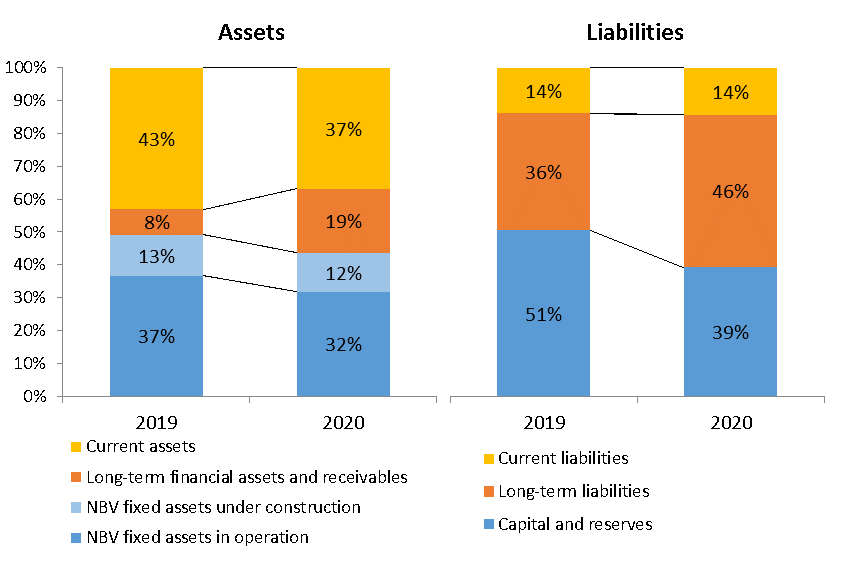
\includegraphics[width=0.7\linewidth]{figures/Figure-5-1} 

}

\caption{(ref:Figure-5-1)}\label{fig:Figure-5-1}
\end{figure}

\begin{infobox}

\begin{left}
\textbf{Spotlight}

On the assets side, the shares of NBV of fixed assets in operations and
of current assets fell by -5 and -6 percent points, respectively. In the
meantime the share of long-term financial assets and receivables rose by
+12 percentage points, mainly due to large under-recoveries from 2020 to
be charged in future years.

On the liabilities side, the share of capital and reserves fell by -11
percentage points (-€1.1 billion) mainly due to the recording of losses
in 2020. In the meantime, the share of long-term liabilities rose by a
+11 percentage points as several ANSPs contracted new loans or drew down
from existing loan facilities in order to respond to liquidity issues
and continue invest in priority projects. Short and long-term borrowings
rose by +€2.5 billion in 2020 (+134\%).

Although the level of capex was reduced by -26\% (-€0.4 billion), it
still represents €1 billion of expenditures.

\end{left}

\begin{right}

\begin{center}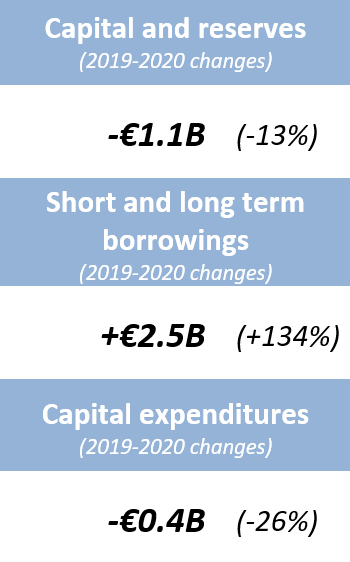
\includegraphics[width=0.9\linewidth]{figures/Figure-5-2} \end{center}

\end{right}

\end{infobox}

\hypertarget{covid_2}{%
\section{Financial indicators calculated from ANSPs ACE data
submissions}\label{covid_2}}

The current ratio, cash-on-hand days, and equity ratio can be calculated
using balance sheet information submitted for ACE at the total ANS
level. For more details on how these ratios have been defined for the
purposes of this analysis, along with their limitations, please refer to
Section 3.4 of the ACE 2019 report. More detailed analysis of changes in
these indicators will be provided in the ACE 2020 benchmarking report.

Figures below show the 1st quartile\footnote{To calculate the average
  value of the 1st and 3rd quartiles over the 2015-2019 period,
  quartiles are first calculated for each year individually (with
  possible differences in sample composition if some ANSP data are
  missing for some years). The yearly ratios are then averaged into a
  single value.}, the Pan-European system average\footnote{The
  Pan-European system average is a weighted average.} and the 3rd
quartile of these three indicators and the changes between the average
for the 2015-2019 period and the year 2020\footnote{As mentioned in
  introduction to this section, HCAA, LVNL and MUAC are excluded from
  all charts. Concerning the current ratio, Fintraffic ANS is also
  excluded for 2015-2016, and DCAC Cyprus for 2015-2018, due to missing
  data. For the cash-on-hand days indicator, ENAIRE is excluded since
  the reporting of cash in ENAIRE ACE submissions does not reflect the
  actual cash available from centralized cash management at ENAIRE Group
  level.}.

\begin{infobox}

\begin{left-narrow}

(ref:Figure-5-3) Changes in ANSPs balance sheet structure (2019-2020)

\begin{center}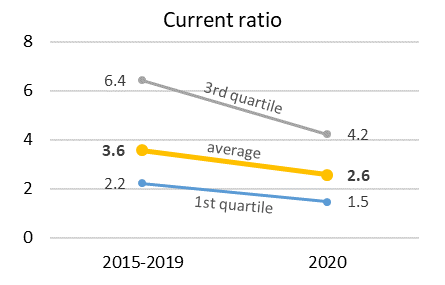
\includegraphics[width=1\linewidth]{figures/Figure-5-3} \end{center}

\begin{center}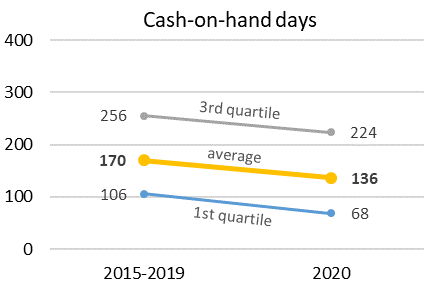
\includegraphics[width=1\linewidth]{figures/Figure-5-4} \end{center}

\begin{figure}

{\centering 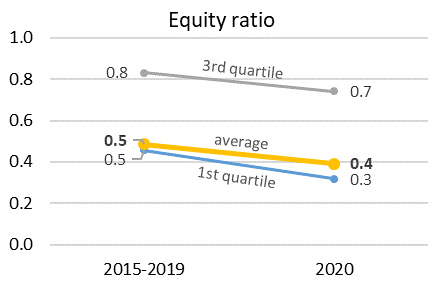
\includegraphics[width=1\linewidth]{figures/Figure-5-5} 

}

\caption{(ref:Figure-5-3)}\label{fig:figure21-bis}
\end{figure}

\end{left-narrow}

\begin{right-wide}
The current ratio measures the ability of a company to pay its
short-term debt obligations with its current assets. A value of more
than 1 suggests financial well-being for the organisation, as it can
settle its short-term debt obligations with its current assets.

In 2020, the average current ratio at Pan-European level amounted to
2.6, which is down by about -28\% compared to the 2015-2019 period.

Cash-on-hand days measures the length of time a company can pay its
operating costs from its cash reserves.

In 2020, the average cash-on-hand days at Pan-European level amounted to
136 days, which is 34 days (or -20\%) lower than over the 2015-2019
period.

The equity ratio measures the share of a company's balance sheet (total
assets or total liabilities) which is financed by equity. A high ratio
can indicate a relatively strong position in case of economic downturn
since the company will have less debt to reimburse and might also be
able to obtain loans more easily.

In 2020, the average equity ratio at Pan-European level amounted to 0.4,
down by -19\% compared to the 2015-2019 period.

\end{right-wide}

\end{infobox}

\hypertarget{covid_3}{%
\section{Cash flow indicators calculated from ANSPs financial
statements}\label{covid_3}}

Free cash flow is an indicator widely used by other aviation industry
stakeholders. Here it is presented at an organisational level, based on
the information reported in ANSPs' financial statements. Depending on
the organisational set up of ANSPs, this information may cover a wider
scope of activities than the scope reported in the ACE submissions for
``Total ANS.'' In the case of DFS, the financial reporting standards
used to establish route charges and for ACE reporting (regulatory
accounting) are also different from the reporting standards used in DFS
financial statements (IFRS). The free cash flow to revenues ratio
provides a representation of the cash generated by operations (after
accounting for capital investments) which is available to repay
creditors or pay dividends and interests to investors. It can therefore
be broken down in two elements: a) the net cash from operating
activities and b) the capital expenditures (CAPEX). Dividing these
ratios by revenues allows an easier interpretation of the indicators
when looking at organisations of different size.

(ref:Figure-5-6) 2019-2020 trends in free cash flow to revenues ratio at
ANSP level

\begin{figure}

{\centering 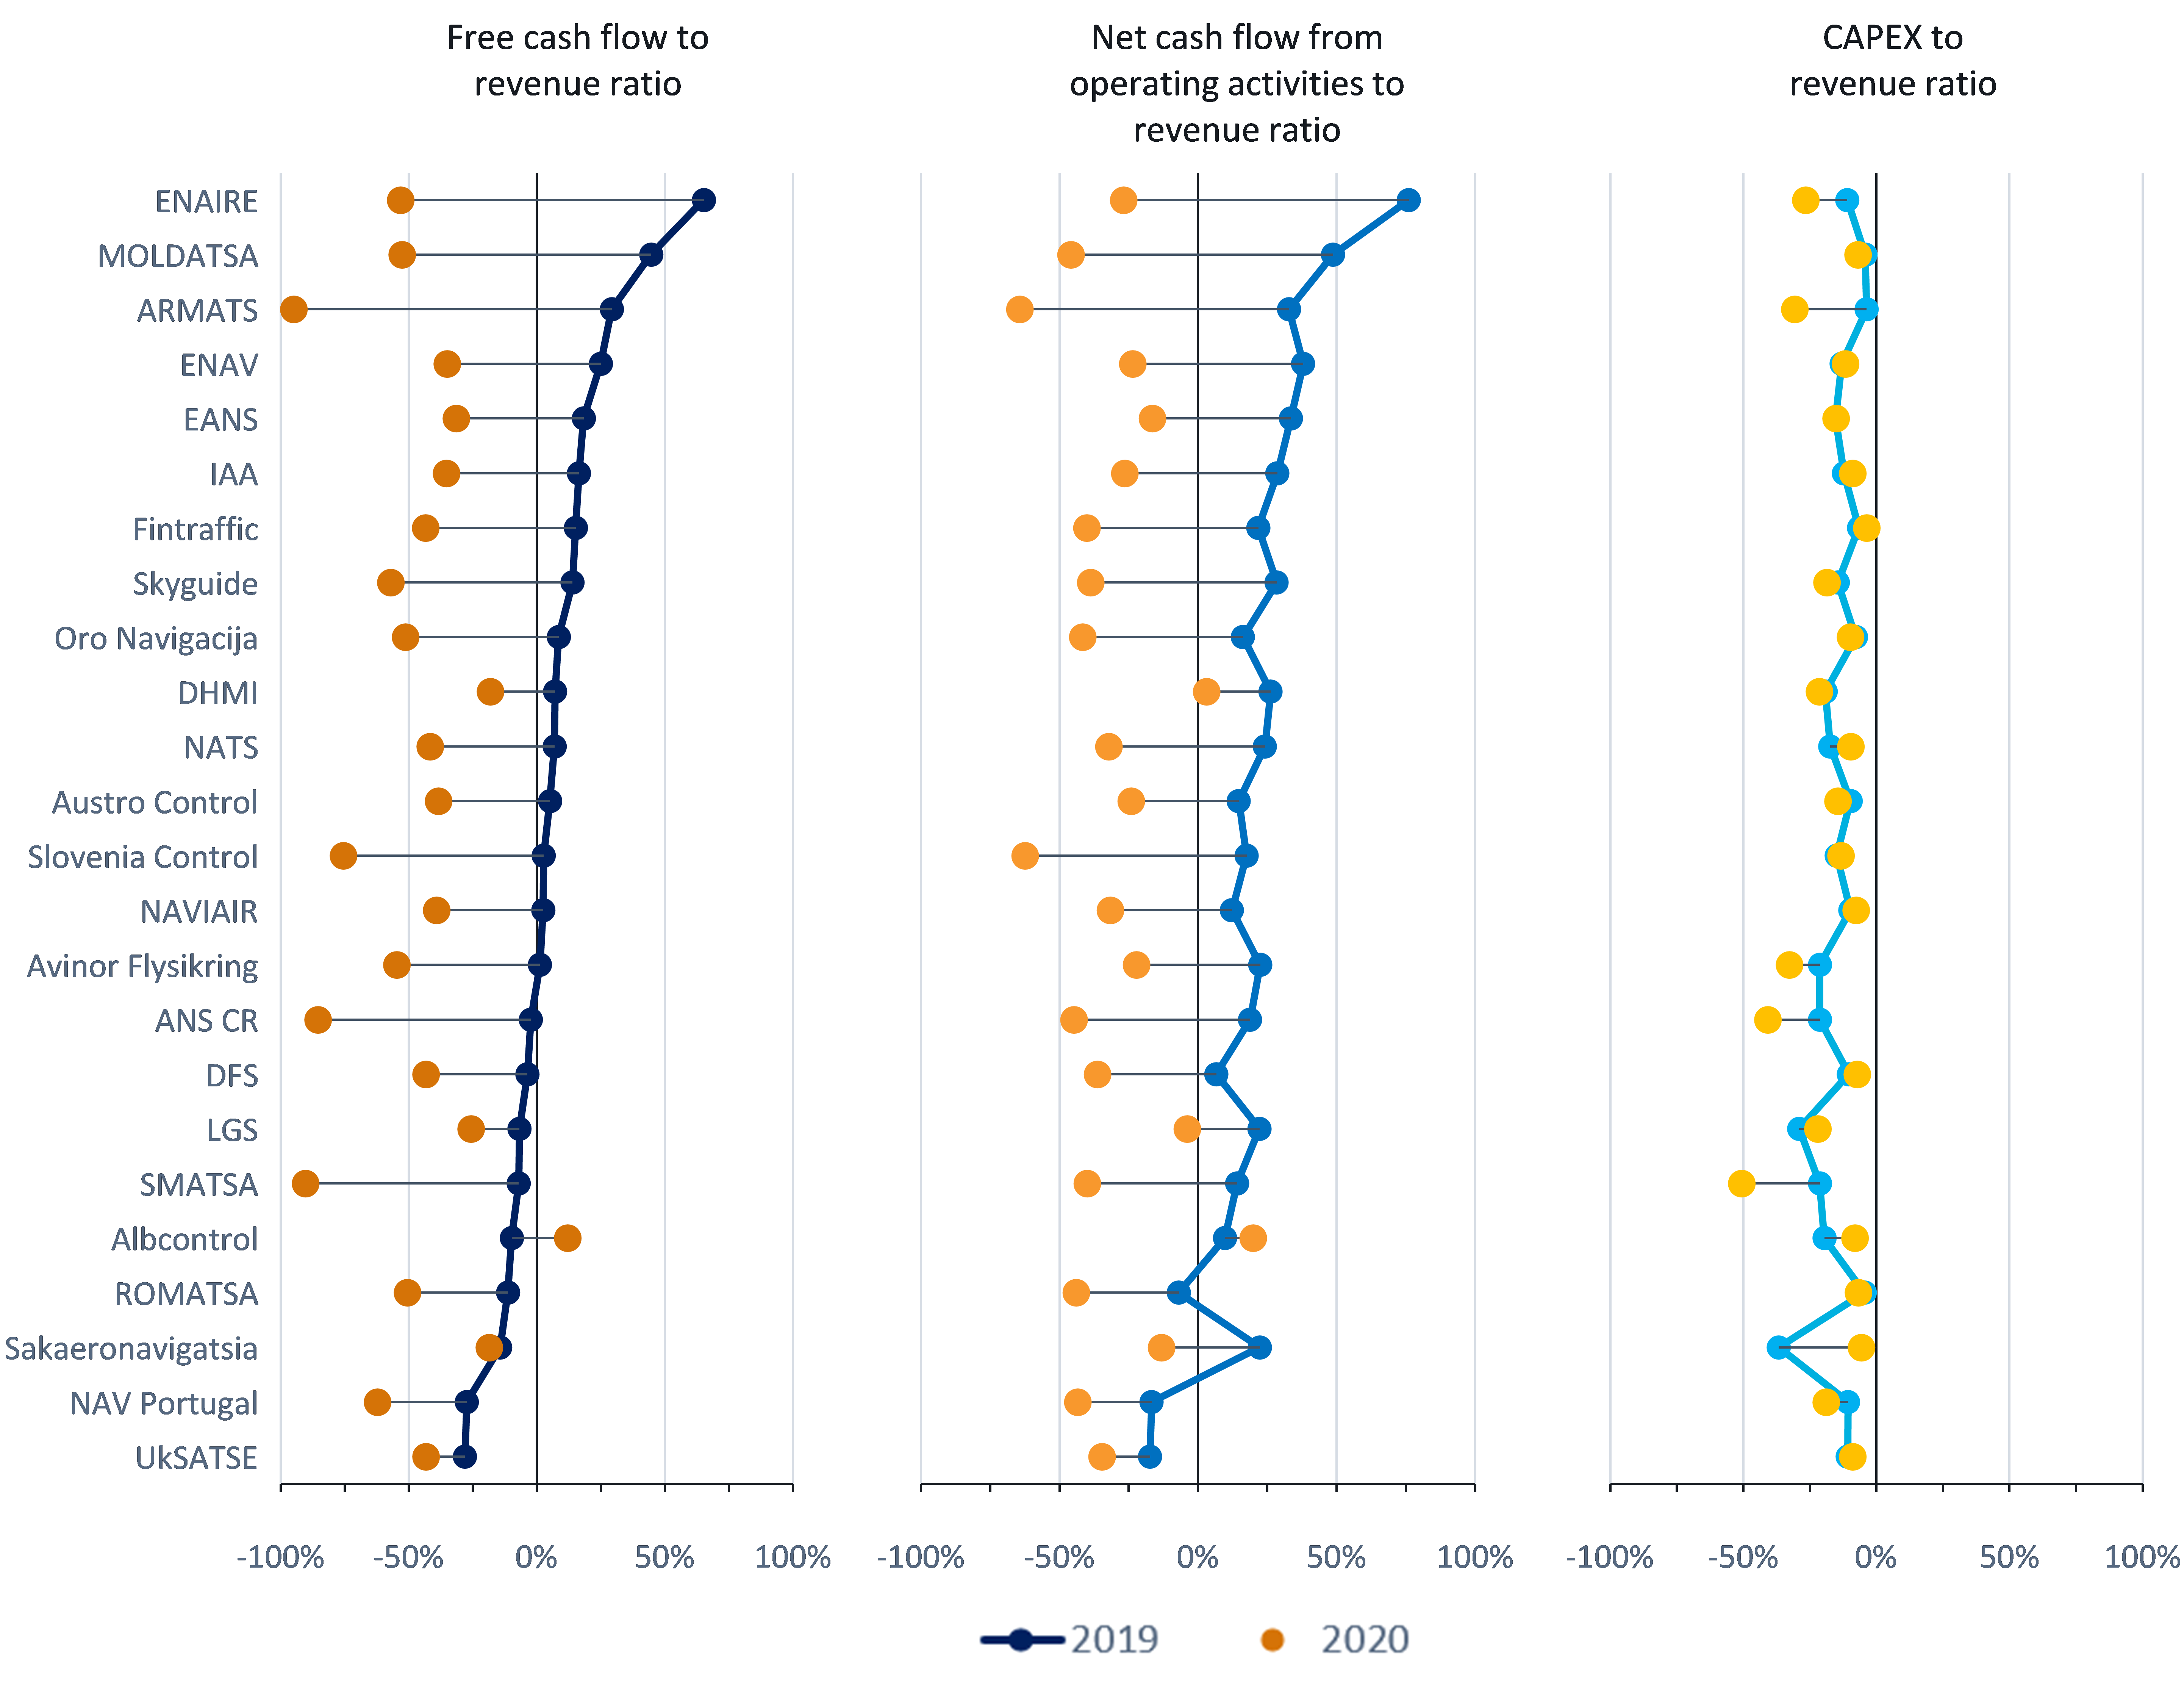
\includegraphics[width=0.7\linewidth]{figures/Figure-5-6} 

}

\caption{(ref:Figure-5-6)}\label{fig:Figure-5-6}
\end{figure}

Figure @ref(fig:Figure-5-6) shows the 2019-2020 changes in free cash
flow to revenues ratio (and its components) at ANSP level for 24 ANSPs
for which data is publically available at the time of writing this
report\footnote{Figure @ref(fig:Figure-5-6) is sourced from the ANSP
  Financial Dashboard produced by the EUROCONTROL Aviation Intelligence
  Unit. All data from this dashboard has been collected from ANSPs' most
  recent financial statements. For more details, see:
  \url{https://ansperformance.eu/economics/finance/}.}.

Whereas 15 of these ANSPs had a positive ratio in 2019, all ANSPs
analysed (with the exception of Albcontrol) have a negative ratio in
2020. Although changes in the free cash flow are mainly driven by
changes in the net cash flow from operating activities (see Figure
@ref(fig:Figure-5-6)), it is interesting to note that when the free cash
flow was negative in 2019, it was in several cases due to relatively
large capital expenditures during the year (e.g.~in 2019,
Sakaeronavigatsia and LGS respectively invested 37\% and 29\% of their
revenues).

More detailed analysis of changes in the free cash flow to revenues
ratio will be provided in the ACE 2020 benchmarking report.

\textbf{Spotlight}

The analysis of ANSPs financial indicators shows that the situation
deteriorated on several criteria:

\begin{itemize}
\tightlist
\item
  The ability to cover short-term debt by using current assets was
  reduced by almost one third compared to the 2015-2019 period (current
  ratio falling from 3.6 to 2.6).
\item
  Cash reserves at the end of 2020 were sufficient to cover 136 days of
  operating expenses (34 days less than over the 2015-2019 period). When
  interpreting this indicator, it is important to consider the fact that
  loans contracted but not fully used in 2020 appear as cash in the
  balance sheet.
\item
  The equity ratio was around 0.4 at the end of 2020, which is lower
  than the 0.5 measured over the 2015-2019 period. This reduction
  results from the combination of a) lower capital reserves due to
  losses incurred in 2020 and b) the increase in borrowings.
\end{itemize}

Based on a sample of 24 ANSPs, the net cash flow from operating
activities in 2020 became negative (-€1.5 billion compared to €2.0
billion in 2020). When also considering the cash outflow for capital
expenditures, the free cash flow amounted to -€2.2 billion in 2020. Free
Cash Flow (24 ANSPs)

\begin{center}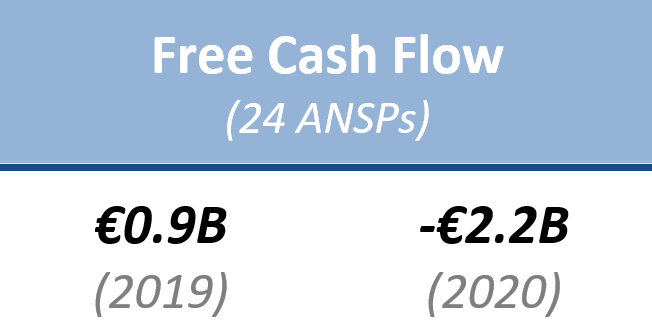
\includegraphics[width=1\linewidth]{figures/Figure-5-7} \end{center}

\hypertarget{disclaimer}{%
\chapter*{Disclaimer}\label{disclaimer}}
\addcontentsline{toc}{chapter}{Disclaimer}

\begin{infobox}
The Performance Review Unit (PRU) has made every effort to ensure that
the information and analysis contained in this document are as accurate
and complete as possible. Should you find any errors or inconsistencies
we would be grateful if you could please bring them to the PRU's
attention. The PRU's e-mail address is
\href{mailto:pru-support@eurocontrol.int}{\nolinkurl{pru-support@eurocontrol.int}}

\end{infobox}

\backmatter
\end{document}
